%! Mode:: "TeX:UTF-8"
%! TEX program = xelatex
\PassOptionsToPackage{quiet}{xeCJK}

\documentclass[withoutpreface,bwprint]{cumcmthesis} %去掉封面与编号页
\usepackage{etoolbox}
\BeforeBeginEnvironment{tabular}{\songti\zihao{-4}}
\usepackage[numbers,super,sort&compress]{natbib}  % 文献管理宏包

% 参考文献标题与目录去重
\makeatletter
\renewcommand{\bibsection}{}

\patchcmd{\thebibliography}{\section*{\refname}}{}{}{}
\patchcmd{\thebibliography}{\section*{\bibname}}{}{}{}

\patchcmd{\thebibliography}{\addcontentsline{toc}{section}{\refname}}{}{}{}
\patchcmd{\thebibliography}{\addcontentsline{toc}{section}{\bibname}}{}{}{}
\patchcmd{\thebibliography}{\addcontentsline{toc}{section}{参考文献}}{}{}{}

\makeatother

\usepackage[framemethod=TikZ]{mdframed}  % 框架宏包
\usepackage{url}  % 网页链接宏包
\usepackage{subcaption}  % 子图宏包
\usepackage{xeCJK} 
\usepackage{listings}
\usepackage{multirow}
\usepackage{mathrsfs}
\usepackage{enumitem}
\usepackage{needspace}
\usepackage{changepage}
\usepackage{booktabs}
\usepackage{longtable}
\usepackage[table]{xcolor}
\usepackage{tabularx}
\usepackage{array}
\usepackage{float}
\usepackage{placeins}
\usepackage{graphicx}
\usepackage{subcaption}
\usepackage{makecell}
\usepackage{xltabular}

\usepackage{algorithm}
\usepackage{algpseudocode}
\usepackage{float}
\floatname{algorithm}{Algorithm}
\renewcommand{\algorithmicrequire}{\textbf{输入：}}
\renewcommand{\algorithmicensure}{\textbf{输出：}}

\usepackage{xurl}
\usepackage{ragged2e}
% 文件名显示命令：不使用 \texttt，且允许下划线处换行
\newcommand{\file}[1]{\begingroup\urlstyle{same}\nolinkurl{#1}\endgroup}


\definecolor{headerblue}{RGB}{210,220,245}
\setlist{itemsep=0.2em, topsep=0.2em}

\definecolor{tablehead}{RGB}{210,220,245}   
\definecolor{tablerow}{RGB}{232,239,247}    % 隔行：浅蓝灰
\definecolor{tableline}{RGB}{95,115,135}    % 横线：深灰蓝

\usepackage[most]{tcolorbox}
\usepackage{enumitem}

\makeatletter
\patchcmd{\thebibliography}{\section*{\refname}}{}{}{}
\patchcmd{\thebibliography}{\section*{\bibname}}{}{}{}
\makeatother

\definecolor{lightbluebg}{RGB}{248,250,252}
\definecolor{deepblue}{RGB}{40,86,145}
\definecolor{lineblue}{RGB}{100,145,195}

\newtcolorbox{highlightbox}{
    colback=lightbluebg,
    colframe=lineblue,
    boxrule=0.7pt,
    arc=2mm,
    left=1.2em,
    right=1.2em,
    top=0.7em,
    bottom=0.6em,
    before skip=0.8em,
    after skip=0.8em
}

%%%%%%%%%%%%%%%%%%%%%%%%%%%%%%%%%%%%%%%%%%%%%%%%%%
%参考文献设置

\makeatletter
% 如果模板里用 \section*{\refname} 来做无编号标题，就把它去掉：
\patchcmd{\thebibliography}
  {\section*{\refname}}   % 查找这一句
  {}                       % 替换为空
  {}{}                     % 成功/失败都不报错
% 如果模板里用 \chapter*{\bibname}（report/book 类）也同理：
\patchcmd{\thebibliography}
  {\chapter*{\bibname}}
  {}
  {}{}
% 对于 natbib 可能单独调用了 \bibsection，也一并清空：
\renewcommand{\bibsection}{}

\makeatother
%引用格式改进
% 让上标引用显示为 \textsuperscript{[1]} 这种带方括号的形式
\setcitestyle{open={[},close={]}}
%%%%%%%%%%%%%%%%%%%%%%%%%%%%%%%%%%%%%%%%%%%%%%%%%%

\lstset{
  basicstyle=\ttfamily\small,
  % …其他你想要的设置
}
% \documentclass[withoutpreface,bwprint]{cumcmthesis} %去掉封面与编号页，电子版提交的时候使用。

\usepackage{titlesec}
\titleformat{\section}{\heiti\bfseries\zihao{4}\centering}{\thesection}{1em}{}
\titleformat{\subsection}{\heiti\bfseries\zihao{-4}}{\thesubsection}{1em}{}
\titleformat{\subsubsection}{\heiti\bfseries\zihao{-4}}{\thesubsubsection}{1em}{}
\titlespacing*{\section}{0pt}{0.5em}{0.3em}
\titlespacing*{\subsection}{0pt}{0.3em}{0.2em}
\titlespacing*{\subsubsection}{0pt}{0.2em}{0.2em}
\AtBeginDocument{\songti\zihao{-4}}
\makeatletter
\patchcmd{\makeothertitle}
  {{\centering \zihao{3}\bfseries \@title\par}}
  {{\centering \zihao{3}\heiti\bfseries \@title\par}}
  {}{}
\patchcmd{\makeothertitle}
  {{\centering \zihao{3}\bfseries \@title\par}}
  {{\centering \zihao{3}\heiti\bfseries \@title\par}}
  {}{}
\makeatother
\newcolumntype{C}{>{\centering\arraybackslash}X}
\newcolumntype{R}{>{\raggedleft\arraybackslash}X}
\newcolumntype{L}{>{\raggedright\arraybackslash}X}

\renewcommand{\abstractname}{\heiti\bfseries\zihao{4}摘要}

\title{考虑绿色限行与动态扰动的城市绿色物流配送调度优化研究}  % 论文标题

\tihao{A}  % 题号
\baominghao{}  % 报名号
\schoolname{}  % 学校
\membera{}  % 队员a
\memberb{}  % 队员b
\memberc{}  % 队员c
\yearinput{2026}
\monthinput{4}
\dayinput{23}

%%%%%%%%%%%%%%%%%%%%%%%%%%%%%%%%%%%%%%%%%%%%%%%%%%%%%%%%%%%%%
%表格字体预设

\AtBeginEnvironment{tabular}{\songti\zihao{-4}}
% 如果你也用 longtable/tabularx，一并加上：
\AtBeginEnvironment{longtable}{\songti\zihao{-4}}
%%%%%%%%%%%%%%%%%%%%%%%%%%%%%%%%%%%%%%%%%%%%%%%%%%%%%%%%%%%%%
%% 正文
\begin{document}

% 前置部分不编号
\pagenumbering{gobble}

\maketitle

\begin{abstract}

针对城市绿色物流配送中混合车队调度、软时间窗约束、时变交通、绿色配送区限行及动态订单扰动等问题，本文以{\heiti 总配送成本最小}为目标，构建{\heiti “静态调度--绿色限行--动态响应”}的递进式优化框架。首先，对订单信息、距离矩阵、客户坐标和时间窗数据进行清洗匹配，统一客户编号、时间和距离口径；随后根据客户坐标识别绿色配送区，并对超容量客户进行任务化拆分，将 $88$ 个有效客户转化为 $237$ 个配送任务，为三类场景建立统一的任务集合和成本评价体系。

对于{\heiti 静态调度问题}，本文建立考虑{\heiti 异质车队、载重与容积双容量约束、软时间窗、时变车速、能耗成本和碳排放成本}的车辆路径优化模型，并采用多随机种子 {\heiti ALNS} 算法求解。无绿色限行时，最优方案启用车辆 $140$ 辆，总配送距离为 $18537.97\,\mathrm{km}$，总配送成本为 $115512.59$ 元。其中固定成本和能耗成本占比较高，迟到成本仅为 $148.58$ 元，说明所得方案在控制运营成本的同时能够较好满足客户时效要求。

对于{\heiti 绿色限行调度问题}，在静态模型基础上加入 $8{:}00$--$16{:}00$ 燃油车禁入绿色配送区约束，并重新优化车辆分配、访问顺序和到达时刻。结果表明，限行后总成本增至 $120037.28$ 元，较无政策情形增加 $4524.70$ 元，增幅为 $3.92\%$；总配送距离仅增加 $94.98\,\mathrm{km}$，说明成本上升主要并非由路径绕行导致，而是来源于等待成本和迟到成本增加。总碳排放量由 $12146.42\,\mathrm{kg}$ 增至 $12292.33\,\mathrm{kg}$，表明在现有新能源运力有限的条件下，{\heiti 单纯实施绿色限行不一定降低企业整体碳排放}。

对于{\heiti 动态事件调度问题}，本文以问题二方案为基准，围绕订单取消、新增订单、配送地址变更和时间窗收紧四类事件，设计{\heiti “状态冻结--任务更新--局部重优化”}的滚动调度策略，并采用 {\heiti LNS--VNS} 算法对受影响路径及邻近路径进行低扰动修复。由于问题三仅评价事件发生后的剩余任务，本文以事件后剩余运营成本作为统一比较口径。四类事件重优化后均较初始响应方案降低成本，节约金额为 $2504.43$--$3484.92$ 元，调整路径数控制在 $4$--$6$ 条之间，说明该策略能够在{\heiti 降低剩余运营成本}的同时有效控制路径扰动。

\vspace{0.3em}
\noindent{\heiti 主要创新与特色：}
\begin{enumerate}[leftmargin=2em,itemsep=0.06em,topsep=0.15em,parsep=0pt]
    \item {\heiti 统一建模框架：}以同一任务集合、车辆集合、约束体系和成本口径贯穿静态调度、绿色限行和动态响应三个问题，保证三类场景结果具有可比性和递进性。

    \item {\heiti 精细成本评价：}将时变车速、载荷修正、油电能耗、碳排放成本、等待成本和迟到惩罚统一纳入路径评估器，能够逐弧计算车辆运行成本并解释成本变化来源。

    \item {\heiti 分场景算法适配：}静态与绿色限行情形采用 ALNS 进行全局路径优化，动态事件采用 LNS--VNS 进行局部重优化，在求解质量、实时响应和路径稳定性之间取得平衡。
\end{enumerate}

\vspace{0.2em}
\noindent{\heiti 关键词：}绿色物流；车辆路径优化；软时间窗；ALNS；LNS--VNS

\end{abstract}

% 目录
\tableofcontents
\clearpage

% 从正文开始重新编号

\pagenumbering{arabic}
\setcounter{page}{1}
\newpage
%%%%%%%%%%%%%%%%%%%%%%%%%%%%%%%%%%%%%%%%%%%%%%%%%%%%%%%%%%%%% 


\section{问题重述}

\subsection{问题背景}

随着电子商务快速发展和城市配送需求持续增长，物流企业面临订单规模扩大、客户分布分散、时效要求提高等现实挑战；同时，城市交通具有明显时段性差异，车辆运行效率、配送成本和能耗水平随交通状态变化而波动。
在“双碳”目标和绿色物流政策推动下，部分城市设立绿色配送区并对燃油车辆实施限行，使配送调度不仅需要兼顾成本与效率，还需满足环保约束。基于此，本文聚焦城市绿色物流配送调度问题，综合考虑客户需求、车辆类型、时间窗约束、时变交通速度及绿色配送区限行政策等因素，建立数学模型并优化不同情境下的车辆调度方案，力求在保障配送服务质量的同时降低企业运营成本与碳排放水平，为城市绿色物流系统的高效运行提供决策依据。

%%%%%%%%%%%%%%%%%%%%%%%%%%%%%%%%%%%%%%%%%%%%%%%%%%%%%%%%%%%%% 

\subsection{问题要求与研究思路}

题目要求基于订单、客户坐标、距离矩阵、时间窗和车队参数，建立综合考虑混合车队、双容量约束、软时间窗、时变车速、能耗排放及绿色限行政策的城市物流配送优化模型。围绕该要求，本文按照“数据预处理--静态调度建模--绿色限行扩展--动态事件响应--结果评价”的思路展开研究，具体分为以下三个环节：

\begin{figure}[htbp]
   \centering
   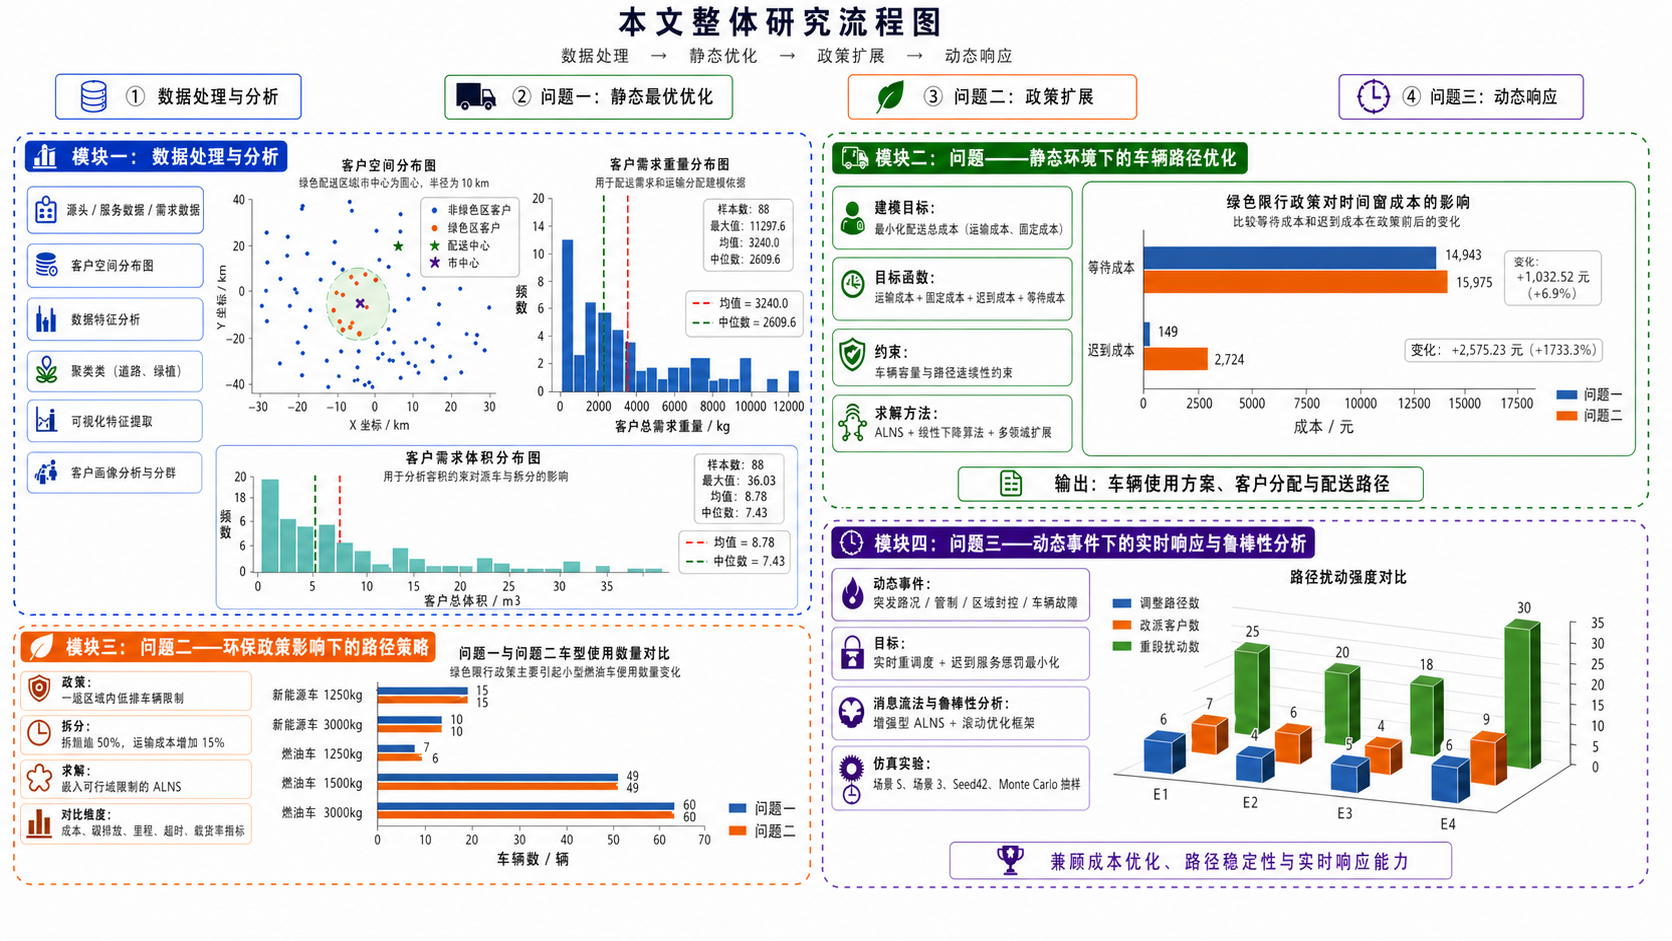
\includegraphics[width=0.98\textwidth]{../figures/paper/liuchengtu0.png}
   \caption{整体研究流程图}
   \label{fig:process}
\end{figure}

\begin{enumerate}[itemindent=2em]
    \item {\heiti 静态环境下的基础调度：}
    对订单、距离矩阵、客户坐标和时间窗数据进行清洗匹配，统一客户编号、时间口径和距离信息，并对超容量客户进行任务化拆分；在此基础上，建立考虑异质车队、双容量约束、软时间窗、时变车速、能耗与碳排放成本的车辆路径优化模型，求解无政策限制下的基准调度方案。

    \item {\heiti 绿色限行政策下的调度重优化：}
    根据客户坐标识别绿色配送区客户，在基础模型中引入 $8{:}00$--$16{:}00$ 燃油车禁入绿色配送区的政策约束，并采用 ALNS 算法重新优化车辆分配、访问顺序和到达时刻，进而分析限行政策对总成本、车辆使用结构、时间窗成本和碳排放水平的影响。

    \item {\heiti 动态事件下的滚动调度：}
    面向订单取消、新增订单、地址变更和时间窗调整等突发事件，构建“状态冻结--任务更新--局部重优化”的动态响应策略；在保留已执行方案的基础上，采用 LNS--VNS 算法修复受影响路径，评价动态扰动下的成本控制、路径扰动和方案稳定性。
\end{enumerate}
%%%%%%%%%%%%%%%%%%%%%%%%%%%%%%%%%%%%%%%%%%%%%%%%%%%%%%%%%%%%% 

\section{模型假设}

为保证模型具有可解性，并使建模口径与题目数据保持一致，本文作如下假设：

\enlargethispage{\baselineskip}
\begin{itemize}[leftmargin=2em,itemsep=0.18em,topsep=0pt,parsep=0pt,partopsep=0pt]
    \item {\heiti 需求确定性假设：}
    客户配送需求由订单数据按客户编号汇总得到，在静态调度和绿色限行情形下视为已知确定量；除问题三所设动态事件外，不考虑其他随机需求扰动。

    \item {\heiti 任务化服务假设：}
    对重量或体积需求超过单车容量上限的客户进行任务化拆分，拆分任务继承原客户的坐标、时间窗和绿色区属性。每个配送任务作为独立服务单元，仅由一辆车完成一次配送；对于同一客户拆分得到的多个任务，均按独立到达与卸货过程处理，服务时间仍取 $20\,\mathrm{min}$。

    \item {\heiti 车辆运行假设：}
    所有车辆均从同一配送中心出发，并在完成所分配任务后返回配送中心；配送过程中不考虑临时换车、中途转运、途中补能及车辆故障等情形。

    \item {\heiti 时间窗与交通假设：}
    时间以 $8{:}00$ 为零点并统一换算为分钟。客户软时间窗作用于开始服务时刻，车辆可提前到达并等待，若开始服务时刻晚于时间窗上界则产生迟到惩罚。车辆行驶速度随交通时段变化，主模型采用各时段速度分布的期望值计算行驶时间，随机交通波动仅在鲁棒性检验中考虑。

    \item {\heiti 能耗与排放假设：}
    车辆油耗或电耗由题目给定的车速--能耗函数确定，并按车辆载荷水平进行修正；能源成本与碳排放成本分别依据对应能源价格、碳排放转换系数和单位碳成本计算。

    \item {\heiti 政策与动态调整假设：}
    绿色配送区依据客户坐标识别。由于题目未提供完整道路网络，本文以车辆到达绿色区客户点的时刻近似表示入区时刻。动态事件发生后，已完成服务及短时间内不可调整的车辆状态保持冻结，仅对后续可调整任务进行局部修复与滚动重优化。
\end{itemize}

%%%%%%%%%%%%%%%%%%%%%%%%%%%%%%%%%%%%%%%%%%%%%%%%%%%%%%%%%%%%% 

\section{符号说明}

\begingroup
\renewcommand{\arraystretch}{1.22}
\arrayrulecolor{tableline}

\begin{xltabular}{0.95\textwidth}{>{\centering\arraybackslash}m{2.6cm}X>{\centering\arraybackslash}m{2.0cm}}
\caption{主要符号说明}
\label{tab:symbols}\\

\toprule
\rowcolor{tablehead}
\textbf{符号} & \textbf{意义} & \textbf{单位} \\
\midrule
\endfirsthead

\multicolumn{3}{c}{续表~\thetable\quad 主要符号说明}\\
\toprule
\rowcolor{tablehead}
\textbf{符号} & \textbf{意义} & \textbf{单位} \\
\midrule
\endhead

\bottomrule
\endfoot

\bottomrule
\endlastfoot

\rowcolor{tablerow}
$i,j,k,r$ & 节点、车辆和车型索引，其中 $0$ 表示配送中心 & 无量纲 \\
$C$ & 有效客户集合，用于订单汇总、坐标识别和任务拆分 & 无量纲 \\
$N,V$ & 配送任务集合与节点集合，$V=\{0\}\cup N$，其中 $0$ 表示配送中心 & 无量纲 \\

\rowcolor{tablerow}
$K,R,K_r$ & 车辆集合、车型集合及车型 $r$ 对应的车辆集合 & 无量纲 \\
$K^F,K^E,G$ & 燃油车集合、新能源车集合与绿色区任务集合 & 无量纲 \\

\rowcolor{tablerow}
$(x_i,y_i)$ & 配送任务 $i$ 继承的原客户二维坐标 & km \\
$q_i^w,q_i^v$ & 配送任务 $i$ 的重量需求与体积需求 & kg；$\mathrm{m}^3$ \\

\rowcolor{tablerow}
$[e_i,l_i],s_i$ & 配送任务 $i$ 的软时间窗与服务时间 & min \\
$Q_k^w,Q_k^v$ & 车辆 $k$ 的最大载重与最大容积 & kg；$\mathrm{m}^3$ \\

\rowcolor{tablerow}
$F_k,m_r$ & 车辆固定启用成本与车型 $r$ 的可用车辆数 & 元；辆 \\
$d_{ij},D$ & 节点 $i$ 到节点 $j$ 的道路距离及距离矩阵 & km \\

\rowcolor{tablerow}
$\bar v(t),\tau_{ij}(t),\bar v_{ij}$ & 期望速度、时变行驶时间与弧 $(i,j)$ 上的等效平均速度 & km/h；min \\
$FPK(v)$ & 速度 $v$ 下燃油车百公里油耗 & L/100 km \\

\rowcolor{tablerow}
$EPK(v)$ & 速度 $v$ 下新能源车百公里电耗 & kWh/100 km \\
$R_{ijk}^w,R_{ijk}^v,\rho_{ijk}$ & 车辆 $k$ 在弧 $(i,j)$ 出发时的剩余载荷与综合载荷率 & kg；$\mathrm{m}^3$；无量纲 \\

\rowcolor{tablerow}
$\phi_F,\phi_E$ & 燃油车与新能源车的载荷修正因子 & 无量纲 \\
$p_f$ & 单位油价 & 元/L \\

\rowcolor{tablerow}
$p_e$ & 单位电价 & 元/kWh \\
$\eta$ & 油耗碳排放转换系数 & kg/L \\

\rowcolor{tablerow}
$\gamma$ & 电耗碳排放转换系数 & kg/kWh \\
$M$ & 大常数 & 无量纲 \\

\rowcolor{tablerow}
$x_{ijk}$ & 若车辆 $k$ 从节点 $i$ 行驶至节点 $j$，则取 $1$，否则取 $0$ & 无量纲 \\
$g_{ik},z_k$ & 任务分配变量与车辆启用变量 & 无量纲 \\

\rowcolor{tablerow}
$A_{ik},B_{ik}$ & 车辆 $k$ 到达配送任务 $i$ 的时刻与开始服务时刻 & min \\
$W_{ik},L_{ik}$ & 车辆 $k$ 在配送任务 $i$ 处的等待时间与迟到时间 & min \\

\rowcolor{tablerow}
$T_k^{\mathrm{dep}},T_k^{\mathrm{ret}}$ & 车辆 $k$ 离开与返回配送中心的时刻 & min \\
$U_{ik}^w,U_{ik}^v$ & 车辆 $k$ 完成配送任务 $i$ 服务后的累计配送重量与体积 & kg；$\mathrm{m}^3$ \\

\rowcolor{tablerow}
$Z$ & 总配送成本 & 元 \\
$c_{ijk}^{\mathrm{ene}},c_{ijk}^{\mathrm{car}}$ & 车辆 $k$ 行驶弧 $(i,j)$ 产生的能源成本与碳排放成本 & 元 \\

\rowcolor{tablerow}
$\widehat C_{\mathrm{ene}},\widehat C_{\mathrm{car}}$ & 路径评估器累计得到的总能源成本与总碳排放成本 & 元 \\
$S,S',S^*$ & 当前解、候选解与当前最优解 & 无量纲 \\

\rowcolor{tablerow}
$N^{done},N^{lock}$ & 已完成任务集合与暂不可调整任务集合 & 无量纲 \\
$N^{rem},N^{new}$ & 尚未服务任务集合与新增订单任务集合 & 无量纲 \\

\rowcolor{tablerow}
$\widetilde N^{rem},N^{dyn}$ & 事件更新后的剩余任务集合与动态待优化任务集合 & 无量纲 \\

$R^0,R^{init},R^*$ & 基准、初始响应与动态重优化方案 & 无量纲 \\

\rowcolor{tablerow}
$K^{aff},K^{nei}$ & 受影响车辆集合与邻近车辆集合 & 无量纲 \\
$K^{sub}$ & 动态优化子问题车辆集合 & 无量纲 \\

\rowcolor{tablerow}
$T_k^{ava}$ & 车辆 $k$ 在动态事件后的最早可用时刻 & min \\
$Z^{dyn},C^{dyn}_{oper}$ & 动态调度目标函数值与事件后剩余任务运营成本 & 元 \\

\end{xltabular}

\arrayrulecolor{black}
\endgroup

%%%%%%%%%%%%%%%%%%%%%%%%%%%%%%%%%%%%%%%%%%%%%%%%%%%%%%%%%%%%% 

\section{数据处理与分析}

\subsection{数据整理与一致性检验}

题目附件包括订单信息、距离矩阵、客户坐标信息和时间窗信息四类数据。本文以客户编号为主键，对订单数据进行汇总，得到各客户的总需求重量与总体积；随后与客户坐标、时间窗和距离矩阵进行匹配，构建统一客户数据表，作为后续建模与算法求解的基础输入。

数据检验结果表明，坐标表和时间窗表共包含 $98$ 个客户点，其中订单数据实际覆盖 $88$ 个客户，即有 $10$ 个客户当日无配送需求。因此，本文将 $98$ 个客户点作为全集客户，用于空间分布分析和绿色区识别；将 $88$ 个有订单需求的客户作为有效客户，用于车辆路径规划。清洗与匹配后，各关键字段均无缺失，数据一致性满足建模要求。

为统一时间计算口径，本文将时间窗转换为以 $8{:}00$ 为零点的分钟数。根据题目补充说明，顺畅、一般和拥堵时段的车辆速度分别服从
\[
N(55.3,0.1^2),\quad N(35.4,5.2^2),\quad N(9.8,4.7^2).
\]
主模型求解时采用各时段速度均值计算行驶时间，并在鲁棒性分析中基于上述分布进行随机扰动。

\subsection{需求特征与绿色区识别}

绿色配送区为以市中心为圆心、半径 $10\,\mathrm{km}$ 的圆形区域。根据题目补充说明，绿色区客户数量应由坐标数据计算确定。设客户 $i$ 的坐标为 $(x_i,y_i)$，则绿色区客户判定条件为
\[
x_i^2+y_i^2\leq 10^2 .
\]

计算结果表明，$98$ 个全集客户中共有 $15$ 个位于绿色配送区；在 $88$ 个有效客户中，共有 $12$ 个绿色区客户。因此，问题二中的绿色限行约束主要作用于这些有效绿色客户及其拆分后的虚拟配送任务。虽然绿色区客户占比不高，但燃油车在 $8{:}00$--$16{:}00$ 期间无法进入该区域，会对车辆分配、到达时刻和路径重组产生直接影响。

从需求分布看，客户重量需求和体积需求均呈现右偏特征，即多数客户需求较小，少数客户需求显著偏大。因此，车辆调度不能采用简单平均分配策略，而需综合考虑车型差异、载重约束、容积约束和客户空间位置。

\subsection{客户任务化处理}

由于部分客户的汇总需求超过单车载重或容积限制，若将其视为单一服务对象，可能导致路径构造不可行。为此，本文对超容量客户进行任务化拆分，将其转化为若干个满足单车容量约束的虚拟配送任务。拆分任务继承原客户的坐标、时间窗和绿色区属性，并作为后续路径优化的基本服务单元。

设有效客户集合为 $C$。对于原客户 $c\in C$，其订单汇总后的重量需求和体积需求分别记为 $\bar q_c^w$ 和 $\bar q_c^v$。若客户 $c$ 的需求超过单车容量上限，则将其拆分为 $h_c$ 个虚拟配送任务，记为 $c_1,c_2,\ldots,c_{h_c}$。为保证需求守恒，拆分结果满足
\begin{equation}
\sum_{\ell=1}^{h_c} q_{c\ell}^w=\bar q_c^w,\qquad
\sum_{\ell=1}^{h_c} q_{c\ell}^v=\bar q_c^v,
\end{equation}
其中，$q_{c\ell}^w$ 和 $q_{c\ell}^v$ 分别表示客户 $c$ 拆分所得第 $\ell$ 个配送任务的重量和体积需求。

经任务化处理后，$88$ 个有效客户被转化为 $237$ 个配送任务。记任务化后的配送任务集合为 $N=\{1,2,\ldots,n\}$，其中 $n=237$。每个配送任务继承其原客户的坐标、时间窗和绿色区属性，并作为后续车辆路径优化的基本服务单元。对于同一客户拆分得到的多个配送任务，本文均视为独立车辆到达与卸货过程，并统一设置服务时间 $s_i=20\,\mathrm{min}$，以避免低估服务时间和时间窗压力。

%%%%%%%%%%%%%%%%%%%%%%%%%%%%%%%%%%%%%%%%%%%%%%%%%%%%%%%%%%%%%

\section{问题一：静态调度模型建立与求解}

\subsection{问题分析}

问题一是在无绿色配送区限行政策条件下的基础静态调度问题。其核心是在完成全部配送任务的前提下，综合确定车辆启用、车型选择、任务分配、任务访问顺序和到达服务时刻，使固定启用成本、能源成本、碳排放成本、等待成本和迟到惩罚成本之和最小。

与经典车辆路径问题\cite{dantzig1959}相比，本题约束耦合更强：车队包含燃油车和新能源车，属于混合车队调度问题\cite{lin2014}；配送任务需求同时受重量和体积双容量约束；软时间窗对应早到等待和晚到惩罚\cite{solomon1987}；时变车速则使访问顺序、出发时刻、能耗和成本相互影响\cite{figliozzi2012,cao2018}。

因此，本文将问题一归结为带异质车队、双容量约束、软时间窗和时变速度的车辆路径优化问题。模型以总配送成本最小为目标，在任务唯一服务、车辆容量、路径连续、时间递推和车队数量限制等约束下求解基础调度方案，并为问题二的绿色限行扩展和问题三的动态重优化提供基准方案。

\begin{figure}[htbp]
  \centering
  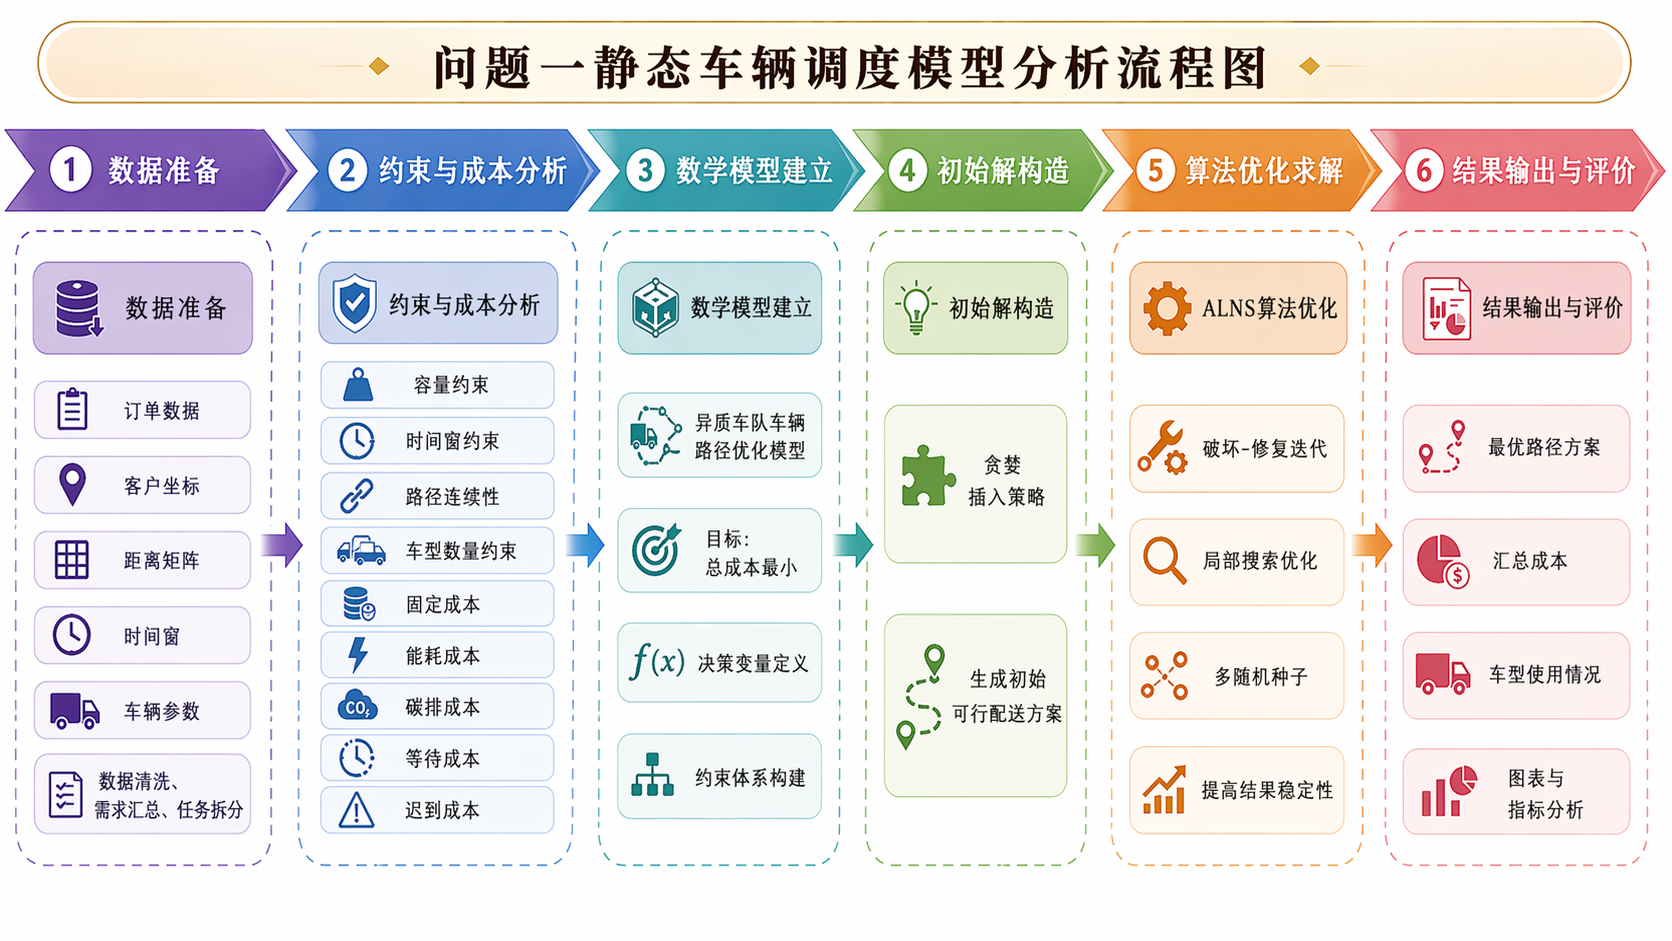
\includegraphics[width = 0.92\textwidth]{../figures/paper/liuchengtu1.png}
  \caption{问题一求解流程图}
  \label{fig:flowchart_q1}
\end{figure}

\subsection{车辆路径调度模型的建立}

为刻画混合车队在时变交通条件下的配送成本，本文借鉴污染路径问题和时变污染路径问题的建模思想\cite{bektas2011,franceschetti2013}，构建带软时间窗和双容量约束的异质车辆路径优化模型。模型以总配送成本最小为目标，综合决定车辆启用、任务分配、任务访问顺序以及各节点到达与服务时刻。

设配送中心为节点 $0$，任务化处理后的配送任务集合为 $N=\{1,2,\cdots,n\}$，其中 $n=237$，节点集合为 $V=\{0\}\cup N$。若配送任务 $i$ 由某一原客户拆分得到，则其坐标、时间窗和绿色区属性继承该原客户。客户任务化后，模型中的节点 $i\in N$ 均表示一个配送任务，而非原始客户点。车辆集合为 $K$，其中 $K^F$ 和 $K^E$ 分别表示燃油车集合与新能源车集合，$K_r$ 表示车型 $r$ 对应的车辆集合。配送任务 $i$ 的需求、时间窗和服务时间分别为 $q_i^w,q_i^v,[e_i,l_i]$ 和 $s_i$，车辆 $k$ 的载重、容积和固定启用成本分别为 $Q_k^w,Q_k^v$ 和 $F_k$，节点间道路距离为 $d_{ij}$。

定义 $x_{ijk}$ 表示车辆 $k$ 是否行驶弧 $(i,j)$，$g_{ik}$ 表示配送任务 $i$ 是否由车辆 $k$ 服务，$z_k$ 表示车辆 $k$ 是否被启用；$A_{ik}$、$B_{ik}$、$W_{ik}$ 和 $L_{ik}$ 分别表示车辆到达时刻、开始服务时刻、等待时间和迟到时间；$T_k^{\mathrm{dep}}$ 和 $T_k^{\mathrm{ret}}$ 分别表示离开与返回配送中心时刻；$U_{ik}^w$ 和 $U_{ik}^v$ 表示完成配送任务 $i$ 服务后的累计配送重量与体积。二元变量定义为
\begin{equation}
g_{ik}=
\begin{cases}
1, & \text{配送任务 } i \text{ 由车辆 } k \text{ 服务},\\
0, & \text{否则},
\end{cases}
\qquad
z_k=
\begin{cases}
1, & \text{车辆 } k \text{ 被启用},\\
0, & \text{否则}.
\end{cases}
\label{eq:gik_zk}
\end{equation}

考虑到车辆速度随交通时段变化，本文以 $8{:}00$ 为时间零点，并采用题目给定速度分布的期望值构造确定性时变速度函数：（由于题目未给出 $17{:}00$ 之后的速度分布，本文延用一般时段期望速度 $35.4\,\mathrm{km/h}$ 作为后续时段速度。）
\begin{equation}
\bar v(t)=
\begin{cases}
9.8,  & t\in[0,60)\cup[210,300),\\
55.3, & t\in[60,120)\cup[300,420),\\
35.4, & t\in[120,210)\cup[420,+\infty).
\end{cases}
\label{eq:speed_function}
\end{equation}

若车辆在时刻 $t$ 从节点 $i$ 出发前往节点 $j$，则行驶时间定义为
\begin{equation}
\tau_{ij}(t)=
\inf\left\{\Delta\geq 0:
\int_t^{t+\Delta}\frac{\bar v(u)}{60}\,du\geq d_{ij}
\right\}.
\label{eq:travel_time}
\end{equation}
其中，$\bar v(u)$ 的单位为 km/h，除以 $60$ 后转化为 km/min。若行驶过程中跨越多个交通时段，则按分段速度累计行驶距离，直至覆盖弧段距离 $d_{ij}$，以更准确刻画时变交通对到达时刻的影响\cite{cao2018}。

题目给出的燃油车百公里油耗和新能源车百公里电耗函数分别为
\begin{equation}
FPK(v)=0.0025v^2-0.2554v+31.75,\qquad
EPK(v)=0.001v^2-0.1v+36.194.
\label{eq:energy_function}
\end{equation}

由于车辆能耗不仅与车速有关，还受载荷水平影响，本文在路径评估器中对每条行驶弧进行逐弧计算。
定义车辆 $k$ 在弧 $(i,j)$ 出发时的综合载荷率为
\begin{equation}
\rho_{ijk}=
\max\left\{
\frac{R_{ijk}^w}{Q_k^w},
\frac{R_{ijk}^v}{Q_k^v}
\right\},
\qquad 0\leq \rho_{ijk}\leq 1,
\label{eq:load_ratio}
\end{equation}
其中，$R_{ijk}^w$ 和 $R_{ijk}^v$ 分别表示车辆在弧 $(i,j)$ 出发时的剩余重量载荷和剩余体积载荷。
根据题意，燃油车满载能耗较空载提高 $40\%$，新能源车满载能耗较空载提高 $35\%$，故设载荷修正因子为
\begin{equation}
\phi_F(\rho_{ijk})=1+0.40\rho_{ijk},
\qquad
\phi_E(\rho_{ijk})=1+0.35\rho_{ijk}.
\label{eq:load_factor}
\end{equation}

在给定车辆路径后，路径评估器根据车辆类型、出发时刻、弧段距离和载荷状态逐弧计算能源成本与碳排放成本。
设
$\bar v_{ij}=60d_{ij}/\tau_{ij}(t)$
为车辆在时刻 $t$ 从节点 $i$ 出发驶向节点 $j$ 时对应的等效平均速度，则单弧能源成本和碳排放成本分别为
\begin{equation}
\begin{aligned}
c_{ijk}^{\mathrm{ene}}
&=
\begin{cases}
\dfrac{d_{ij}}{100}FPK(\bar v_{ij})\phi_F(\rho_{ijk})p_f,
& k\in K^F,\\[6pt]
\dfrac{d_{ij}}{100}EPK(\bar v_{ij})\phi_E(\rho_{ijk})p_e,
& k\in K^E,
\end{cases}\\
c_{ijk}^{\mathrm{car}}
&=
\begin{cases}
\dfrac{d_{ij}}{100}FPK(\bar v_{ij})\phi_F(\rho_{ijk})\eta c_c,
& k\in K^F,\\[6pt]
\dfrac{d_{ij}}{100}EPK(\bar v_{ij})\phi_E(\rho_{ijk})\gamma c_c,
& k\in K^E.
\end{cases}
\end{aligned}
\label{eq:arc_cost}
\end{equation}
其中，$p_f$ 和 $p_e$ 分别为油价和电价，$\eta$ 和 $\gamma$ 分别为燃油与电耗的碳排放转换系数，$c_c$ 为单位碳排放成本。

需要说明的是，能源成本和碳排放成本同时依赖于车辆类型、出发时刻、路径顺序和载荷变化，难以简单表示为固定弧成本。
因此，本文采用“主模型刻画可行域、路径评估器计算行驶成本”的处理方式，将路径评估器逐弧累计得到的能源成本和碳排放成本分别记为
$\widehat C_{\mathrm{ene}}(x,B,U)$ 和 $\widehat C_{\mathrm{car}}(x,B,U)$。
于是，问题一的目标函数为
\begin{equation}
\min Z=
\sum_{k\in K}F_k z_k
+\widehat C_{\mathrm{ene}}(x,B,U)
+\widehat C_{\mathrm{car}}(x,B,U)
+c_w\sum_{k\in K}\sum_{i\in N}W_{ik}
+c_l\sum_{k\in K}\sum_{i\in N}L_{ik}.
\label{eq:objective}
\end{equation}
其中，第一项为车辆固定启用成本，第二、三项分别为能源成本和碳排放成本，第四、五项分别为等待成本和迟到惩罚成本。

模型约束如下。

首先，每个配送任务必须且只能被一辆车服务，且任务服务变量与路径变量保持一致：
\begin{equation}
\left\{
\begin{alignedat}{2}
\sum_{k\in K}g_{ik} &=1,
&\qquad& \forall i\in N,\\
\sum_{\substack{j\in V\\j\ne i}}x_{ijk} &=g_{ik},
&& \forall i\in N,\ k\in K,\\
\sum_{\substack{j\in V\\j\ne i}}x_{jik} &=g_{ik},
&& \forall i\in N,\ k\in K.
\end{alignedat}
\right.
\label{eq:service_flow}
\end{equation}

车辆若被启用，则必须从配送中心出发并最终返回配送中心；未启用车辆不能服务配送任务：
\begin{equation}
\left\{
\begin{alignedat}{2}
\sum_{j\in N}x_{0jk} &=z_k,
&\qquad& \forall k\in K,\\
\sum_{i\in N}x_{i0k} &=z_k,
&& \forall k\in K,\\
g_{ik} &\leq z_k,
&& \forall i\in N,\ k\in K.
\end{alignedat}
\right.
\label{eq:depot_activation}
\end{equation}

车辆载重和容积均不能超过对应车型容量：
\begin{equation}
\left\{
\begin{aligned}
\sum_{i\in N}q_i^w g_{ik} &\leq Q_k^w z_k,\\
\sum_{i\in N}q_i^v g_{ik} &\leq Q_k^v z_k,
\end{aligned}
\right.
\qquad \forall k\in K.
\label{eq:capacity}
\end{equation}

为防止不经过配送中心的孤立子回路，引入累计配送量约束：
\begin{equation}
\left\{
\begin{alignedat}{2}
q_i^w g_{ik} &\leq U_{ik}^w \leq Q_k^w g_{ik},
&\qquad& \forall i\in N,\ k\in K,\\
U_{jk}^w &\geq U_{ik}^w+q_j^w-Q_k^w(1-x_{ijk}),
&& \forall i,j\in N,\ i\ne j,\ k\in K,\\
q_i^v g_{ik} &\leq U_{ik}^v \leq Q_k^v g_{ik},
&& \forall i\in N,\ k\in K,\\
U_{jk}^v &\geq U_{ik}^v+q_j^v-Q_k^v(1-x_{ijk}),
&& \forall i,j\in N,\ i\ne j,\ k\in K.
\end{alignedat}
\right.
\label{eq:subtour_capacity}
\end{equation}

车辆时间递推关系如下：
\begin{equation}
\left\{
\begin{alignedat}{2}
0\leq T_k^{\mathrm{dep}}
&\leq T_k^{\mathrm{ret}}\leq Mz_k,
&\qquad& \forall k\in K,\\
A_{jk}
&\geq T_k^{\mathrm{dep}}+\tau_{0j}(T_k^{\mathrm{dep}})
-M(1-x_{0jk}),
&& \forall j\in N,\ k\in K,\\
A_{jk}
&\geq B_{ik}+s_i+\tau_{ij}(B_{ik}+s_i)
-M(1-x_{ijk}),
&& \forall i,j\in N,\ i\ne j,\ k\in K,\\
T_k^{\mathrm{ret}}
&\geq B_{ik}+s_i+\tau_{i0}(B_{ik}+s_i)
-M(1-x_{i0k}),
&& \forall i\in N,\ k\in K.
\end{alignedat}
\right.
\label{eq:time_recursion}
\end{equation}

软时间窗作用于配送任务的开始服务时刻。车辆可以提前到达并等待，若开始服务时刻晚于时间窗上界，则产生迟到惩罚：
\begin{equation}
\left\{
\begin{alignedat}{2}
B_{ik} &\geq A_{ik}-M(1-g_{ik}),
&\qquad& \forall i\in N,\ k\in K,\\
B_{ik} &\geq e_i-M(1-g_{ik}),
&& \forall i\in N,\ k\in K,\\
W_{ik} &\geq B_{ik}-A_{ik}-M(1-g_{ik}),
&& \forall i\in N,\ k\in K,\\
L_{ik} &\geq B_{ik}-l_i-M(1-g_{ik}),
&& \forall i\in N,\ k\in K,\\
0\leq W_{ik} &\leq Mg_{ik},\qquad
0\leq L_{ik}\leq Mg_{ik},
&& \forall i\in N,\ k\in K.
\end{alignedat}
\right.
\label{eq:soft_time_window}
\end{equation}

每种车型的启用数量不能超过题目给定车队规模：
\begin{equation}
\sum_{k\in K_r}z_k\leq m_r,\qquad \forall r\in R.
\label{eq:fleet_size}
\end{equation}

最后，变量取值约束为
\begin{equation}
\left\{
\begin{alignedat}{2}
x_{ijk},g_{ik},z_k &\in \{0,1\},
&\qquad& \forall i,j\in V,\ i\ne j,\ k\in K,\\
A_{ik},B_{ik},W_{ik},L_{ik},U_{ik}^w,U_{ik}^v
&\in \mathbb{R}_{+},
&& \forall i\in N,\ k\in K,\\
T_k^{\mathrm{dep}},T_k^{\mathrm{ret}}
&\in \mathbb{R}_{+},
&& \forall k\in K.
\end{alignedat}
\right.
\label{eq:variable_domain}
\end{equation}

综上，式 \eqref{eq:objective} 为总配送成本最小化目标函数，
式 \eqref{eq:service_flow}--\eqref{eq:variable_domain}
分别刻画任务服务与流平衡、车辆启用、双容量限制、子回路消除、
时间递推、软时间窗、车型数量及变量取值约束，由此完成问题一静态车辆路径调度模型的建立。

\subsection{模型求解}

问题一同时涉及异质车队选择、任务分配、路径排序、双容量约束、软时间窗约束以及时变速度下的成本评估，属于约束耦合较强的组合优化问题。若采用精确算法直接求解，变量规模和约束数量较大，难以满足实际调度效率要求。因此，本文借鉴 Shaw 提出的大邻域搜索思想\cite{shaw1998}，并参考 Ropke 和 Pisinger 提出的自适应大邻域搜索框架\cite{ropke2006}，设计基于 ALNS 的多算子大邻域搜索算法进行求解。

算法采用“初始解构造--破坏修复--路径评估--概率接受--权重更新--多种子择优”的框架。先根据需求规模、时间窗紧迫度和可服务车型构造任务优先级，并用贪婪插入生成初始可行解；再通过破坏修复调整任务分配与访问顺序，并调用路径评估器计算时刻和成本。候选解按模拟退火准则接受\cite{kirkpatrick1983}，算子权重随搜索表现动态更新。流程见算法\ref{alg:alns}。

\begin{algorithm}[H]
\caption{基于 ALNS 的车辆配送路径优化算法}
\label{alg:alns}
\footnotesize
\begin{algorithmic}[1]
\Require 配送任务集合 $N$，车辆集合 $K$，距离矩阵 $D$，任务需求 $q_i^w,q_i^v$，时间窗 $[e_i,l_i]$，随机种子集合 $\mathcal{S}$，最大迭代次数 $I_{\max}$，运行时间上限 $t_{\max}$
\Ensure 最优配送方案 $S^*$ 及其总成本 $Z(S^*)$

\State 对订单、时间窗、距离矩阵和车辆参数进行预处理；
\State 构建路径评估器 $\operatorname{Eval}(\cdot)$，设定破坏算子集合 $\mathcal{D}$ 与修复算子集合 $\mathcal{R}$；
\State 初始化全局最优解 $S^*\gets \varnothing$，$Z(S^*)\gets +\infty$；

\For{每个随机种子 $s\in\mathcal{S}$}
    \State 设置随机种子 $s$，采用贪婪插入策略生成初始可行解 $S$；
    \State 初始化破坏算子和修复算子的选择权重；
    \State 令当前种子最优解 $S^{best}\gets S$，温度 $T\gets T_0$；
    
    \For{$iter=1$ to $I_{\max}$ 且运行时间未超过 $t_{\max}$}
        \State 按当前权重从 $\mathcal{D}$ 和 $\mathcal{R}$ 中选择破坏算子 $d$ 与修复算子 $r$；
        \State 使用 $d$ 从当前解 $S$ 中移除部分任务，得到部分解 $\bar S$；
        \State 使用 $r$ 将被移除任务重新插入 $\bar S$，生成候选解 $S'$；
        \State 调用 $\operatorname{Eval}(S')$ 计算成本，并检验容量、时间窗、车型数量及相应场景约束；
        
        \If{$S'$ 可行}
            \State $\Delta Z\gets Z(S')-Z(S)$；
            \If{$\Delta Z<0$ 或以概率 $\exp(-\Delta Z/T)$ 接受}
                \State $S\gets S'$；
            \EndIf
            
            \If{$Z(S)<Z(S^{best})$}
                \State $S^{best}\gets S$；
            \EndIf
        \EndIf
        
        \State 根据候选解表现更新破坏算子与修复算子的选择权重；
        \State 按 $T\gets \alpha T$ 更新温度；
    \EndFor
    
    \If{$Z(S^{best})<Z(S^*)$}
        \State $S^*\gets S^{best}$；
    \EndIf
\EndFor

\State \Return $S^*$。
\end{algorithmic}
\end{algorithm}

\FloatBarrier

破坏阶段设置随机移除、最差任务移除、相关任务移除和整条路径移除，用于增强扰动、调整高成本任务、重构相近任务群和优化车辆启用结构；修复阶段采用最小增量成本插入、regret 插入和时间窗优先插入，将任务重新插入可行路径。各算子初始权重相同，迭代中按产生优质解或可接受改进解的表现获得奖励，并据此更新选择权重。

为降低初始解构造和随机算子选择对结果的影响，本文采用多随机种子独立运行策略。对不同随机种子得到的候选解进行统一可行性检验，并在所有可行解中选取总配送成本最低的方案作为问题一最终结果。最终输出车辆使用方案、配送路径、到达与开始服务时刻，以及固定成本、能源成本、碳排放成本、等待成本和迟到惩罚成本等指标。

\subsubsection{算法参数设置}

为保证实验结果的可复现性，本文统一设定问题一 ALNS 算法的主要参数，见表 \ref{tab:p1_alns_params}。算法采用多随机种子独立运行，并在通过任务覆盖、车型数量、载重容量、容积容量和软时间窗计罚规则检验的可行方案中，选取总配送成本最低者作为最终调度结果。

\begin{table}[H]
\centering
\caption{问题一 ALNS 求解参数设置}
\label{tab:p1_alns_params}
\renewcommand{\arraystretch}{1.16}
\setlength{\tabcolsep}{8pt}
\arrayrulecolor{tableline}
\small
\begin{tabular}{
>{\centering\arraybackslash}p{0.18\textwidth}
>{\centering\arraybackslash}p{0.45\textwidth}
>{\centering\arraybackslash}p{0.26\textwidth}}
\toprule
\rowcolor{tablehead}
\textbf{参数} & \textbf{含义} & \textbf{取值} \\
\midrule
$\mathcal{S}$ & 多随机种子集合 & $\{1,7,21,42,66,88,100\}$ \\
\rowcolor{tablerow}
$I_{\max}$ & 最大迭代次数 & $300$ \\
$t_{\max}$ & 单个随机种子的运行时间上限 & $180\,\mathrm{s}$ \\
\rowcolor{tablerow}
$T_0$ & 模拟退火初始温度 & $2000$ \\
$\alpha$ & 降温系数，按 $T\leftarrow \alpha T$ 更新 & $0.985$ \\
\rowcolor{tablerow}
$p$ & 每次破坏操作移除的任务比例 & $[0.04,0.16]$ \\
$c_w$ & 单位等待成本 & $20/60$ 元/min \\
\rowcolor{tablerow}
$c_l$ & 单位迟到惩罚成本 & $50/60$ 元/min \\
$c_c$ & 单位碳排放成本 & $0.65$ 元/kg \\
\bottomrule
\end{tabular}
\end{table}

在候选解接受阶段，设当前解和候选解分别为 $S$ 与 $S'$。若 $Z(S')<Z(S)$，则直接接受候选解；否则以概率
\[
P=\exp\left(-\frac{Z(S')-Z(S)}{T}\right)
\]
接受该候选解，并在每轮迭代后按 $T\leftarrow \alpha T$ 更新温度。该机制使算法在搜索初期保留一定的全局探索能力，后期逐步转向稳定收敛。

问题二在相同求解框架下进一步嵌入绿色配送区限行检验：若燃油车在 $8{:}00$--$16{:}00$ 到达绿色区任务，则该插入方案判定为不可行。每次候选解生成后，均调用路径评估器重新计算时间可行性与成本构成，以保证算法评价口径与目标函数一致。


\subsection{结果分析}

基于上述参数设置，本文对问题一进行多随机种子求解，并统计各次运行的成本水平与可行性，结果如表 \ref{tab:p1_alns_stability} 所示。

\begin{table}[H]
\centering
\caption{问题一 ALNS 多随机种子求解稳定性验证}
\label{tab:p1_alns_stability}
\renewcommand{\arraystretch}{1.15}
\setlength{\tabcolsep}{6pt}
\arrayrulecolor{tableline}
\small
\begin{tabular}{c c c c c c}
\toprule
\rowcolor{tablehead}
\textbf{种子数} & \textbf{最优种子} & \textbf{最优成本/元} & \textbf{平均成本/元} & \textbf{变异系数/\%} & \textbf{可行率/\%} \\
\midrule
7 & 100 & 115512.59 & 116559.92 & 0.613 & 100 \\
\bottomrule
\end{tabular}
\arrayrulecolor{black}
\end{table}

由表 \ref{tab:p1_alns_stability} 可知，问题一在 7 个随机种子下均得到可行解，可行率为 $100\%$；目标函数值的变异系数为 $0.613\%$，说明算法结果对随机种子的敏感性较低，具有较好的求解稳定性。其中，随机种子为 $100$ 时取得最低总成本 $115512.59$ 元，故本文选取该方案作为问题一最终调度方案。

问题一最终优化结果如表 \ref{tab:p1_result_summary} 所示。

\begin{table}[H]
\centering
\caption{问题一最终优化结果汇总}
\label{tab:p1_result_summary}
\renewcommand{\arraystretch}{1.16}
\setlength{\tabcolsep}{8pt}
\arrayrulecolor{tableline}
\small
\begin{tabular}{
>{\centering\arraybackslash}p{0.22\textwidth}
>{\centering\arraybackslash}p{0.18\textwidth}
>{\centering\arraybackslash}p{0.22\textwidth}
>{\centering\arraybackslash}p{0.18\textwidth}
}
\toprule
\rowcolor{tablehead}
\textbf{指标} & \textbf{数值} & \textbf{指标} & \textbf{数值} \\
\midrule
最优随机种子 & 100 & 配送任务数 & 237 \\
\rowcolor{tablerow}
使用车辆数 & 140 & 总配送距离/km & 18537.97 \\
总成本/元 & 115512.59 & 固定成本/元 & 56000.00 \\
\rowcolor{tablerow}
能耗成本/元 & 36526.07 & 碳排放成本/元 & 7895.17 \\
等待成本/元 & 14942.76 & 迟到成本/元 & 148.58 \\
\rowcolor{tablerow}
任务覆盖 & 全部覆盖 & 车型数量 & 满足约束 \\
\bottomrule
\end{tabular}
\arrayrulecolor{black}
\end{table}

由表 \ref{tab:p1_result_summary} 可知，问题一最优方案共启用车辆 $140$ 辆，完成 $237$ 个配送任务，总配送距离为 $18537.97\,\mathrm{km}$，总成本为 $115512.59$ 元。其中，固定成本为 $56000.00$ 元，能耗成本为 $36526.07$ 元，二者是总成本的主要来源；等待成本为 $14942.76$ 元，说明软时间窗对路径时序安排具有明显影响；迟到成本仅为 $148.58$ 元，表明方案能够较好地控制服务延误。

\subsubsection{调度结果可行性与合理性验证}

本文采用贪婪插入策略构造初始可行解，并通过 ALNS 的破坏--修复机制持续改进。最终方案通过了任务覆盖、车型数量和时间窗成本三类检验：一是 $237$ 个配送任务全部被覆盖，未出现漏送或重复服务；二是各车型启用数量均未超过题目给定车队规模；三是迟到成本仅占总成本的 $0.13\%$，说明算法在降低总成本的同时较好地控制了服务延误。

从车型启用结构看，方案呈现“大容量车辆主导、新能源车辆充分利用、小型车辆补充服务”的特征。燃油车 $3000\,\mathrm{kg}$、$1500\,\mathrm{kg}$ 和 $1250\,\mathrm{kg}$ 型分别启用 $60$、$49$ 和 $6$ 辆；新能源车 $3000\,\mathrm{kg}$ 和 $1250\,\mathrm{kg}$ 型分别启用 $10$ 和 $15$ 辆，均被全部启用。

为进一步说明调度方案的可执行性，本文选取部分代表性车辆路径，列出车辆访问顺序、任务到达时刻和开始服务时刻，如表 \ref{tab:p1_route_time_example} 所示。其中，任务节点括号内的两个时间分别表示车辆到达该配送任务的时刻和开始服务时刻。

\begin{table}[H]
\centering
\caption{问题一部分车辆路径与到达时间示例}
\label{tab:p1_route_time_example}
\renewcommand{\arraystretch}{1.18}
\setlength{\tabcolsep}{4pt}
\arrayrulecolor{tableline}
\footnotesize
\begin{tabularx}{\textwidth}{
>{\centering\arraybackslash}p{1.25cm}
>{\centering\arraybackslash}p{1.55cm}
>{\raggedright\arraybackslash}p{3.3cm}
>{\raggedright\arraybackslash}X
>{\centering\arraybackslash}p{1.2cm}
>{\centering\arraybackslash}p{1.2cm}}
\toprule
\rowcolor{tablehead}
\textbf{路径编号} & \textbf{车型} & \centering\textbf{访问顺序} 
& \centering\textbf{各任务到达 $\rightarrow$ 开始服务时刻} 
& \textbf{距离/km} & \textbf{成本/元} \\
\midrule

R003 & 燃油3000 & 
0 $\rightarrow$ 32\_1 $\rightarrow$ 75\_2 $\rightarrow$ 45\_1 $\rightarrow$ 0 &
32\_1：10:42 $\rightarrow$ 13:08；
75\_2：13:47 $\rightarrow$ 14:25；
45\_1：15:18 $\rightarrow$ 15:37 &
174.47 & 993.29 \\

\rowcolor{tablerow}
R013 & 新能源3000 & 
0 $\rightarrow$ 87\_1 $\rightarrow$ 39\_3 $\rightarrow$ 57\_4 $\rightarrow$ 0 &
87\_1：10:49 $\rightarrow$ 11:18；
39\_3：13:07 $\rightarrow$ 14:08；
57\_4：16:07 $\rightarrow$ 16:07 &
213.21 & 611.02 \\

R016 & 新能源1250 &
0 $\rightarrow$ 74\_1 $\rightarrow$ 0 &
74\_1：10:01 $\rightarrow$ 13:11 &
131.67 & 566.19 \\

\rowcolor{tablerow}
R041 & 燃油1500 &
0 $\rightarrow$ 48\_2 $\rightarrow$ 0 &
48\_2：09:28 $\rightarrow$ 16:06 &
71.56 & 742.05 \\

\bottomrule
\end{tabularx}

\vspace{0.3em}
\begin{minipage}{0.96\textwidth}
\footnotesize
注：$0$ 表示配送中心；$32\_1$ 表示客户 $32$ 拆分得到的第 $1$ 个配送任务；
“到达 $\rightarrow$ 开始服务”表示车辆到达配送任务对应客户点后，若早于时间窗下界，则需等待至允许服务时刻后开始服务。
\end{minipage}
\end{table}

由表 \ref{tab:p1_route_time_example} 可见，问题一调度方案能够同时给出车辆访问顺序、任务到达时刻和开始服务时刻。
例如，路径 R003 中车辆于 10:42 到达任务 32\_1，但由于早于该任务允许服务时刻，
需等待至 13:08 后开始服务；路径 R013 中任务 57\_4 的到达时刻与开始服务时刻均为 16:07，
说明该节点无需等待即可服务。由此可见，路径评估器能够正确刻画提前到达等待和按时间窗开始服务的过程。

\subsubsection{成本构成与碳排放分析}

问题一成本构成如图 \ref{fig:p1_cost_structure} 所示。

\begin{figure}[htbp]
   \centering
   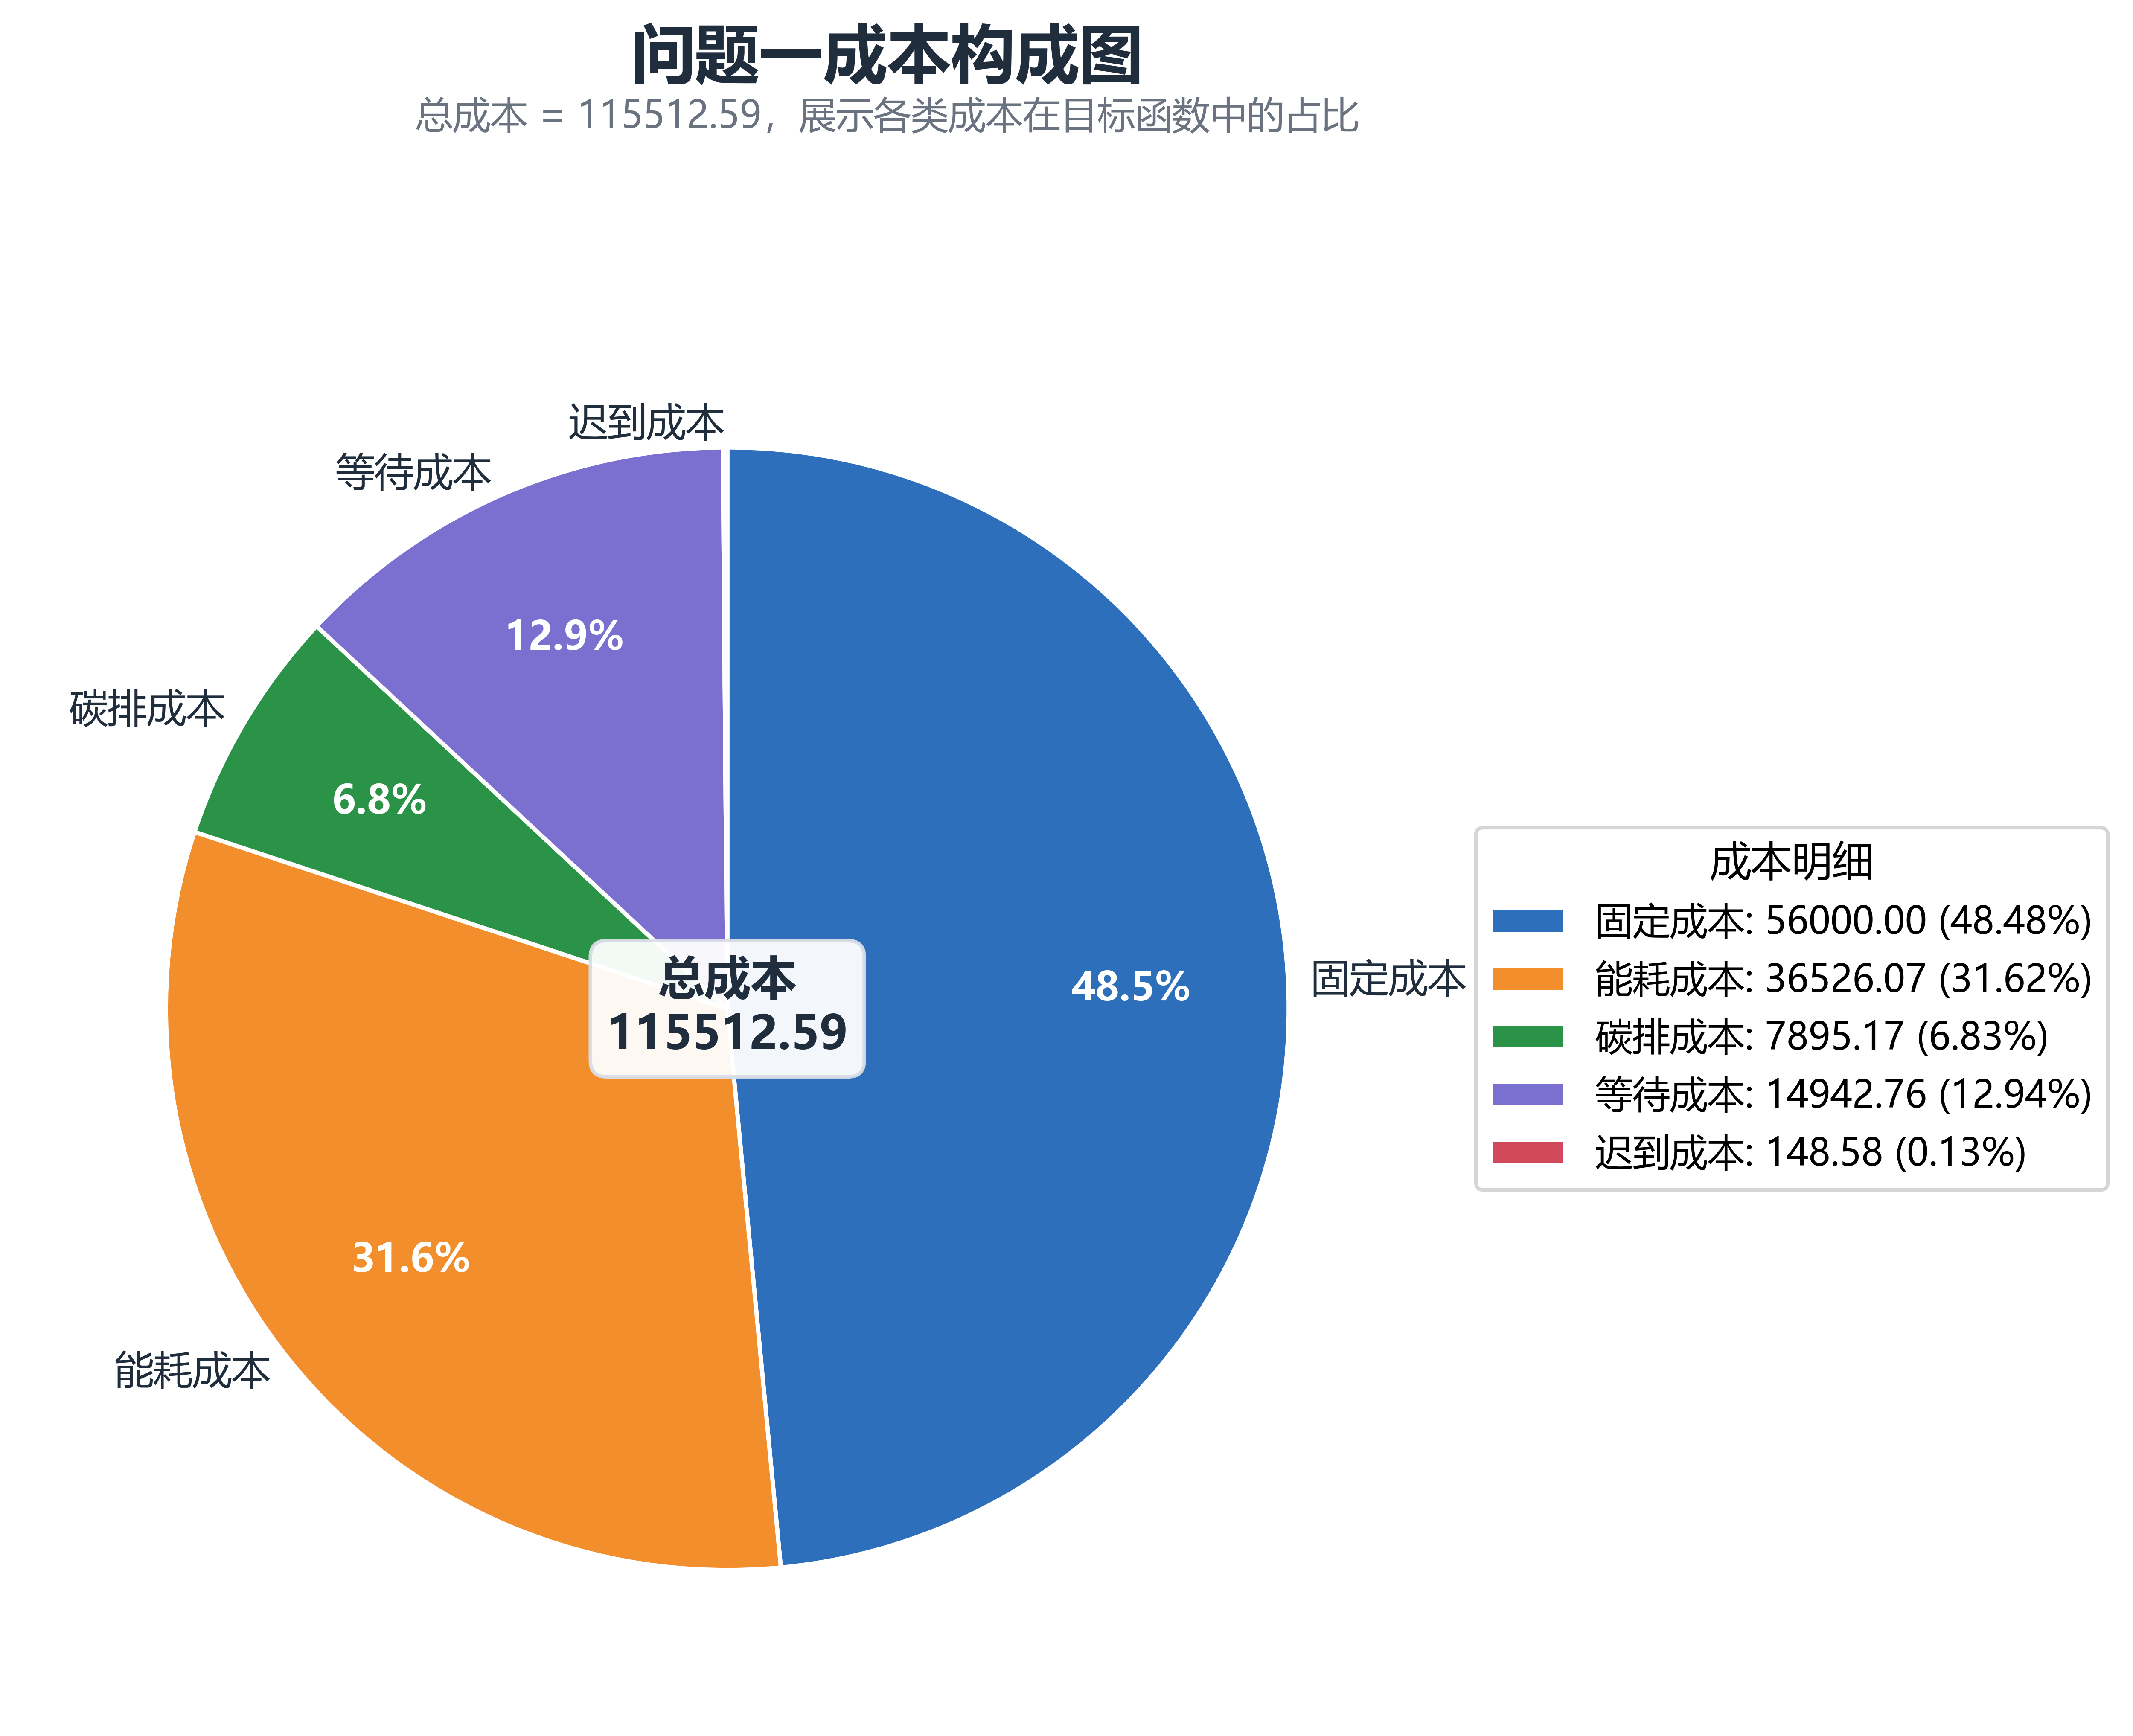
\includegraphics[width = 0.50\textwidth]{../figures/paper/q1_chengben.png}
   \caption{问题一成本构成图}
   \label{fig:p1_cost_structure}
\end{figure}

由图 \ref{fig:p1_cost_structure} 可知，固定成本和能耗成本分别占 $48.48\%$ 和 $31.62\%$，合计超过 $80\%$，是静态调度成本的主要来源。等待成本占 $12.94\%$，碳排放成本占 $6.83\%$，迟到成本仅占 $0.13\%$。

进一步地，根据碳排放成本和单位碳成本可估算问题一方案的总碳排放量。由于单位碳排放成本为 $0.65$ 元/kg，因此有
\[
E_1=\frac{7895.17}{0.65}=12146.42\ \mathrm{kg}.
\]
该结果作为问题二分析绿色配送区限行政策对碳排放影响的基准值。

\subsubsection{路径组织均衡性分析}

\begin{figure}[H]
    \centering
    \begin{subfigure}[b]{0.48\textwidth}
        \centering
        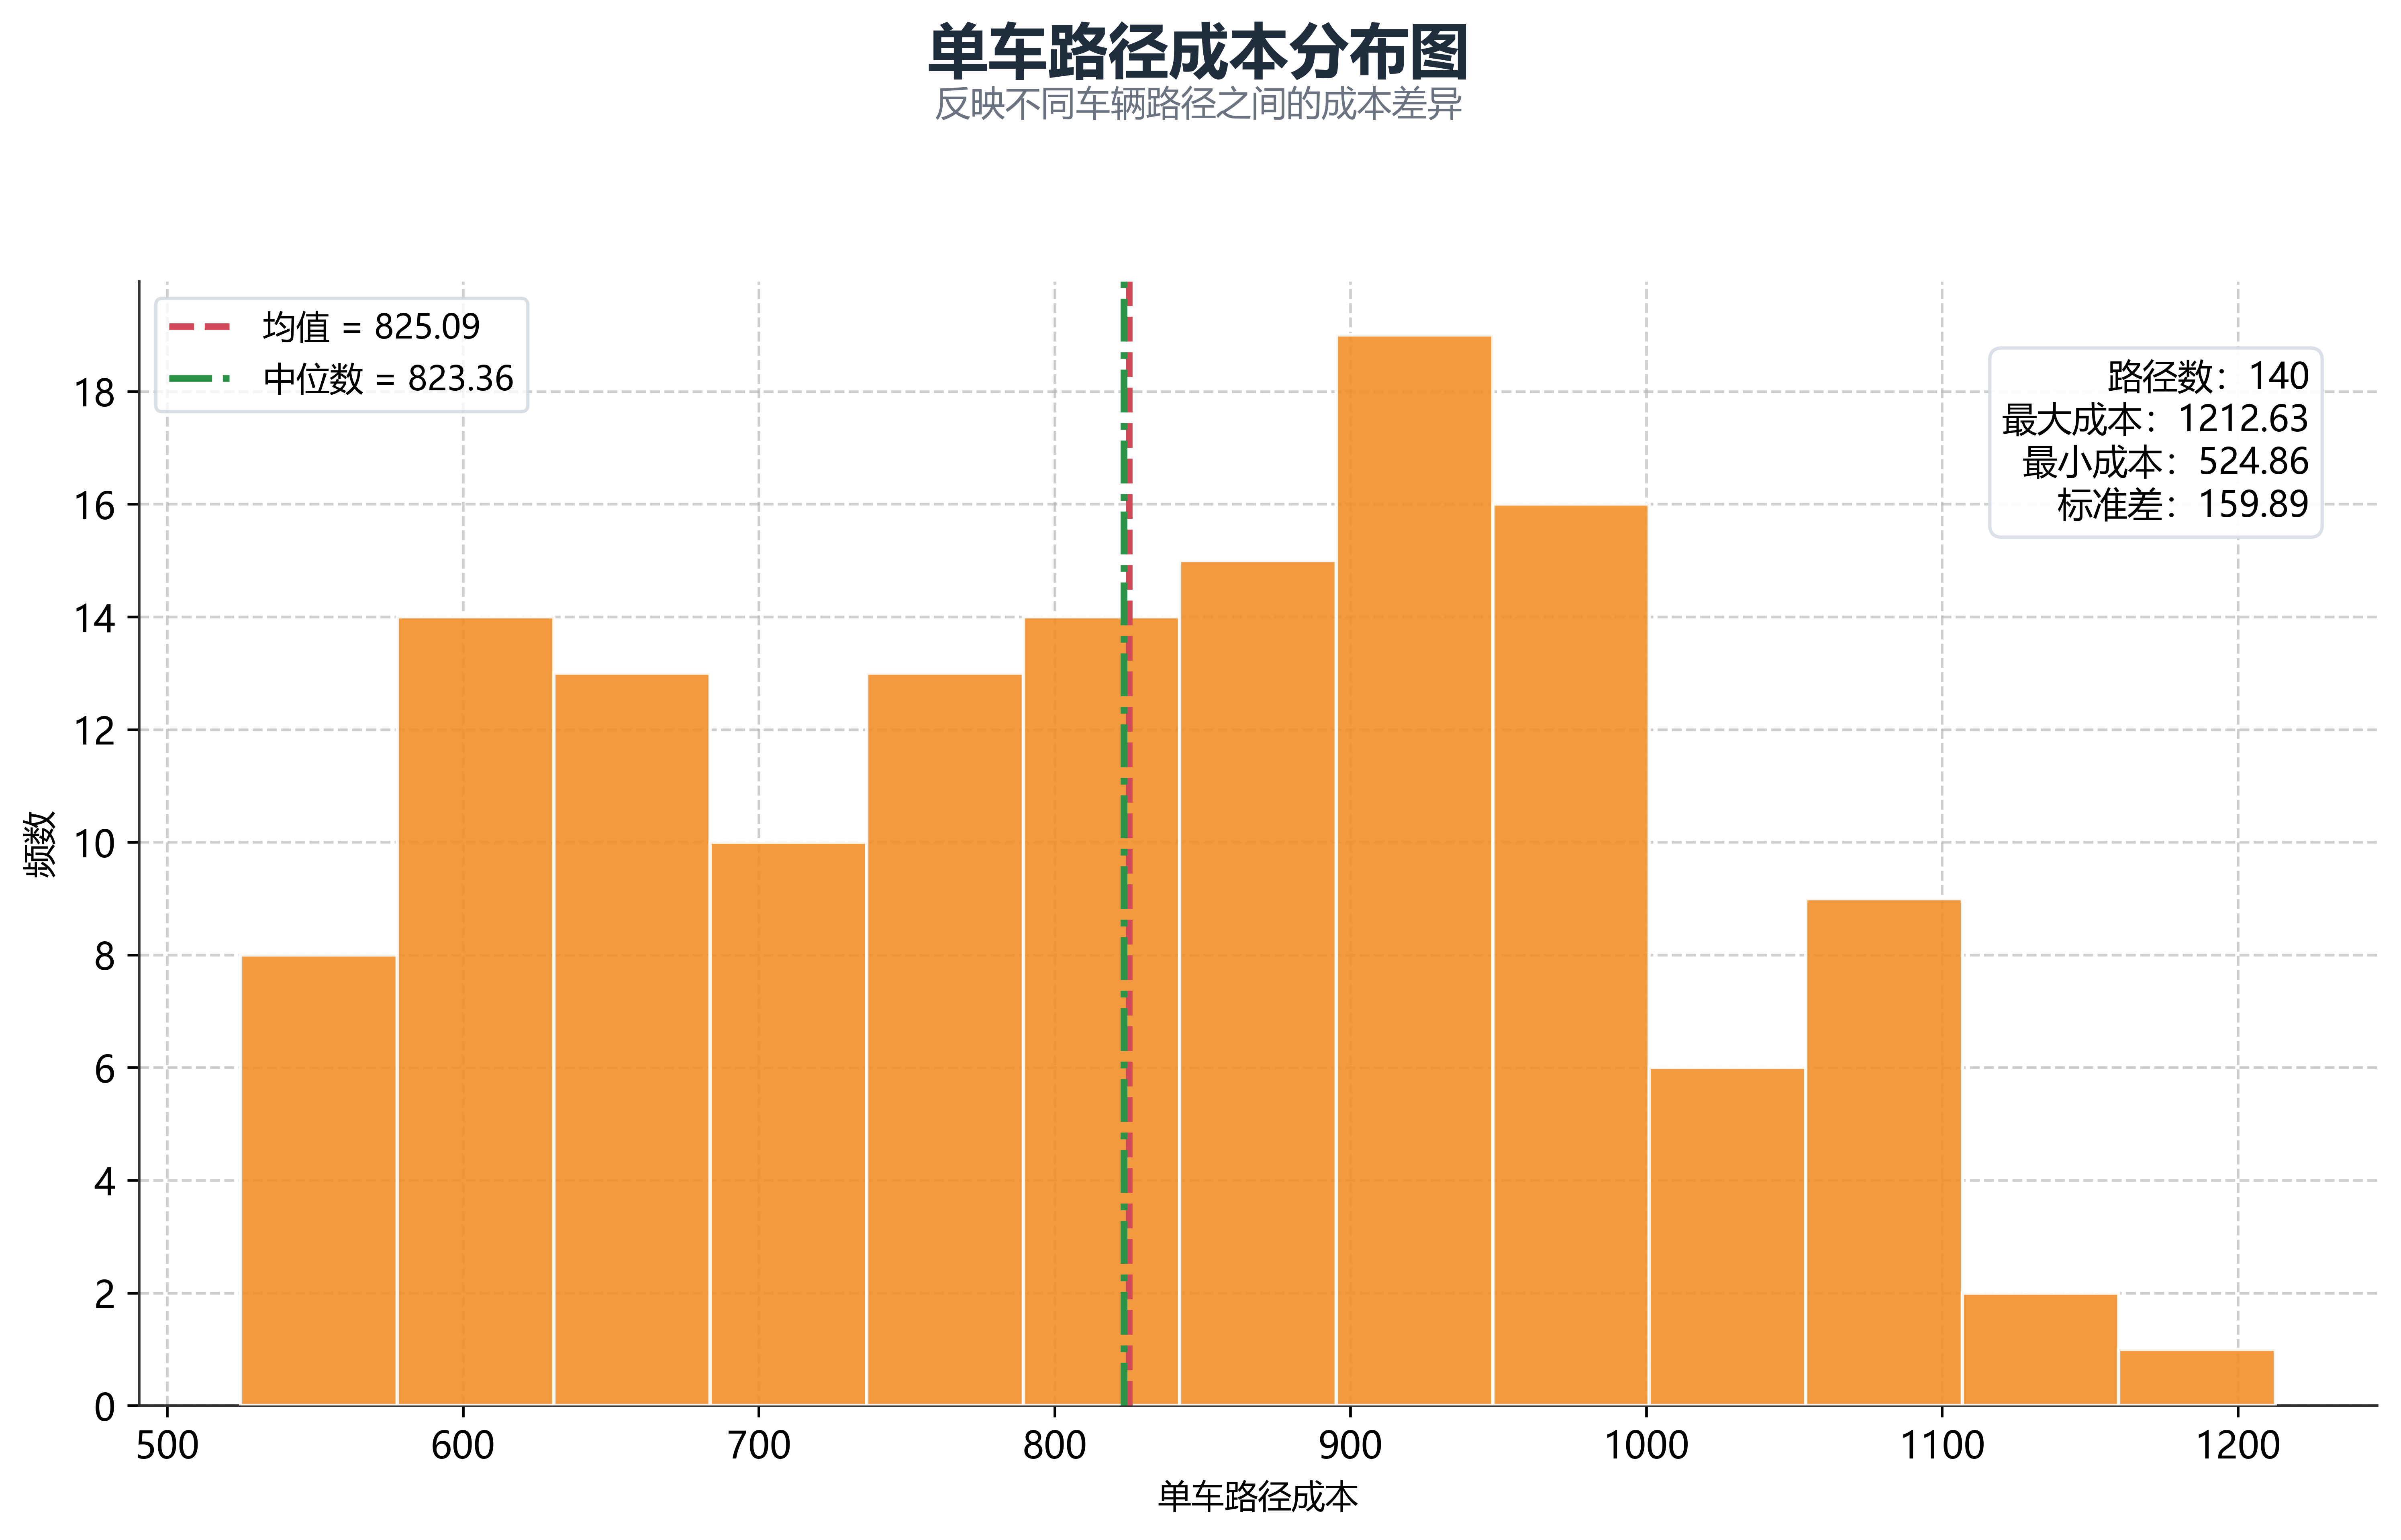
\includegraphics[width=\linewidth]{../figures/paper/p1_route_cost_distribution.png}
        \caption{单车路径成本分布}
        \label{fig:p1_route_cost_distribution}
    \end{subfigure}
    \hfill
    \begin{subfigure}[b]{0.48\textwidth}
        \centering
        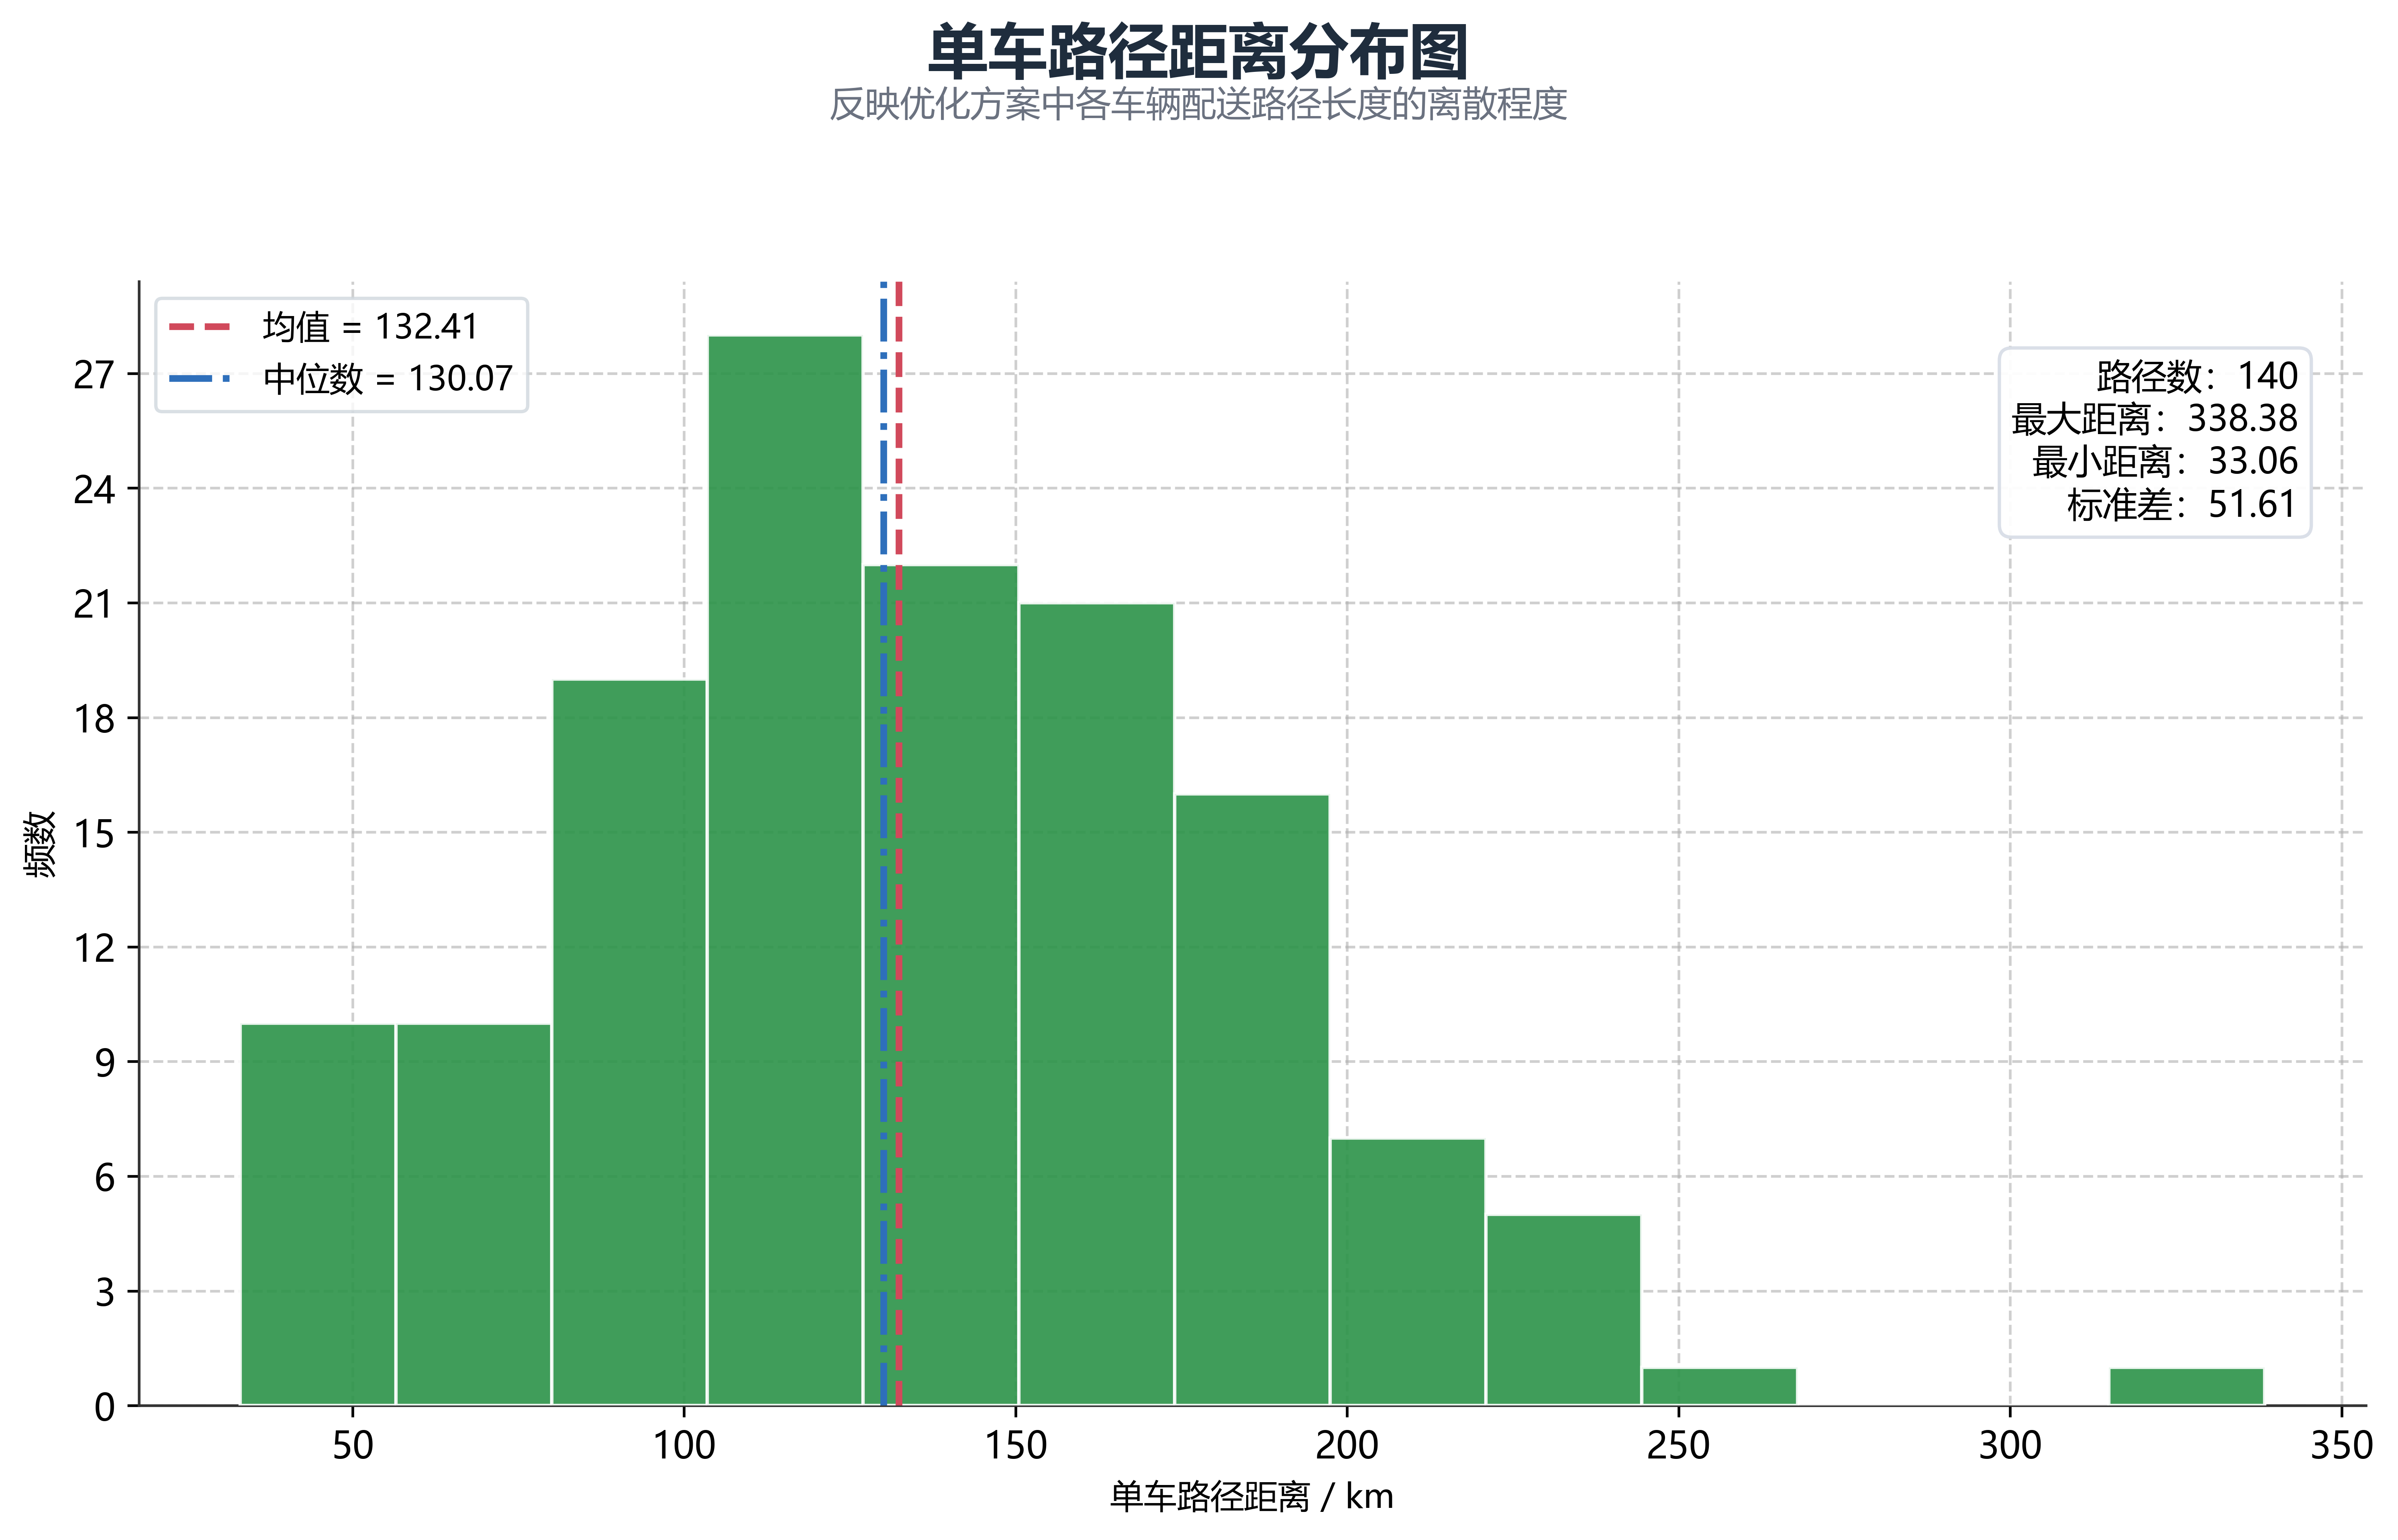
\includegraphics[width=\linewidth]{../figures/paper/p1_route_distance_distribution.png}
        \caption{单车路径距离分布}
        \label{fig:p1_route_distance_distribution}
    \end{subfigure}
    \caption{问题一单车路径成本与距离分布}
    \label{fig:p1_route_distribution}
\end{figure}

为考察路径组织均衡性，本文统计单车路径成本与距离，结果如图 \ref{fig:p1_route_distribution} 所示。单车成本主要集中在 $600$--$1000$ 元，平均值 $825.09$ 元，中位数 $823.36$ 元；单车距离主要集中在 $100$--$200\,\mathrm{km}$，平均值 $132.41\,\mathrm{km}$，中位数 $130.07\,\mathrm{km}$，说明路径规模较集中。

此外，问题一方案的平均单车服务任务数为
\[
\frac{237}{140}=1.69.
\]
该数值相对较小，主要是由于任务化拆分后，部分配送任务仍受到载重、容积、时间窗和空间分布等多重约束限制，难以进一步合并。因此，较高的车辆启用数量并非单纯由算法搜索不足造成，而是多重约束共同作用下形成的可行调度结果。

综上，问题一所得方案能够完成全部配送任务，并满足容量、路径连续性、车型数量和软时间窗计罚要求。结果表明，固定成本和能耗成本是总成本的主要来源，软时间窗约束对路径时序安排具有明显影响，而迟到成本较低，说明所设计算法能够有效控制配送延误。该方案可作为问题二绿色限行扩展和问题三动态重优化的基准方案。

%%%%%%%%%%%%%%%%%%%%%%%%%%%%%%%%%%%%%%%%%%%%%%%%%%%%%%%%%%%%% 

\section{问题二：绿色限行调度模型建立与求解}

\subsection{问题分析}

问题二是在问题一静态调度模型基础上加入绿色配送区限行政策后的再优化问题。根据题意，$8{:}00$--$16{:}00$ 期间燃油车禁止进入以市中心为圆心、半径 $10\,\mathrm{km}$ 的绿色配送区，因此问题一所得方案在该政策下可能不再可行，需要重新调整车辆分配、任务访问顺序和到达时刻。

与问题一相比，问题二的配送任务需求、车辆容量、时间窗和成本构成均保持不变，主要变化在于燃油车对绿色区任务的服务时段受到限制，使可行解空间进一步压缩。因此，问题二可归结为带绿色配送区限行约束的异质车队车辆路径优化问题，重点是在新能源车辆优先服务、燃油车辆延后服务和路径重组之间进行权衡，并评估限行政策对总成本、车辆结构和碳排放水平的影响\cite{lin2014,bektas2011,franceschetti2013}。

\subsection{绿色配送区识别与限行约束建立}

在问题一模型基础上，问题二进一步识别绿色配送区客户，并将其拆分后得到的配送任务纳入绿色区任务集合。由于配送任务继承原客户坐标，绿色区任务集合可表示为
\begin{equation}
G=\left\{i\in N\mid x_i^2+y_i^2\leq 10^2\right\}.
\label{eq:green_area_set}
\end{equation}

对于 $i\in G$ 的配送任务，新能源车辆可在任意时段进入并完成配送；若由燃油车服务，则其到达时刻不得早于 $16{:}00$。以 $8{:}00$ 为时间零点，$16{:}00$ 对应 $480$ min。沿用问题一中的任务分配变量 $g_{ik}$ 和到达时刻变量 $A_{ik}$，对任意 $i\in G$、$k\in K^F$，建立限行约束：
\begin{equation}
A_{ik}\geq 480-M(1-g_{ik}),\qquad i\in G,\ k\in K^F,
\label{eq:green_policy_constraint}
\end{equation}
其中，$M$ 为充分大的正常数。当 $g_{ik}=1$ 时，式 \eqref{eq:green_policy_constraint} 退化为 $A_{ik}\geq 480$，表示燃油车只能在 $16{:}00$ 后到达绿色区任务；当 $g_{ik}=0$ 时，该约束自动松弛。

需要说明的是，题目附件仅提供客户坐标和点间道路距离矩阵，未给出完整道路网络及车辆穿越绿色区边界的具体位置。因此，本文以车辆到达绿色区任务所对应客户点的时刻近似表示进入绿色配送区的时刻。该处理与数据粒度相匹配，能够保证绿色区任务在限行时段内不由燃油车直接服务。若考虑更保守的调度情形，可引入安全缓冲时间 $\delta$，将约束改写为
\[
A_{ik}\ge 480+\delta-M(1-g_{ik}),\qquad i\in G,\ k\in K^F.
\]
本文在缺少完整路网数据的条件下取 $\delta=0$。

\subsection{模型求解}

问题二在问题一 ALNS 求解框架的基础上进行扩展，仍采用“初始解构造--破坏修复--路径评估--概率接受--多随机种子择优”的搜索流程\cite{shaw1998,ropke2006}。与问题一相比，问题二的配送任务需求、车辆容量、时间窗和成本评价口径保持不变，主要区别在于算法在初始解构造、任务重插入和候选解可行性检验中嵌入绿色配送区限行规则。

具体而言，对于绿色区任务，算法在插入阶段优先尝试将其分配至新能源车辆路径；若候选插入方案由燃油车服务绿色区任务，则进一步检查其到达时刻。若燃油车到达绿色区任务的时刻早于 $16{:}00$，则该插入位置被判定为不可行；仅当其到达时刻不早于 $16{:}00$ 时，才允许进入候选解。通过该方式，绿色限行约束被直接嵌入 ALNS 的可行性检验过程，从而避免生成违反政策约束的路径方案。

为降低随机初始化和邻域算子选择对结果的影响，本文仍采用多随机种子独立运行策略，随机种子集合设为
\[
\mathcal{S}=\{1,7,21,42,66,88,100\}.
\]
各随机种子下独立执行 ALNS 搜索，并在所有满足容量、时间窗、车型数量和绿色限行约束的可行方案中，选取总成本最低者作为问题二最终调度结果。

为保证问题一与问题二结果具有可比性，问题二沿用问题一的随机种子集合、最大迭代次数、运行时间上限、降温系数和成本评价口径。考虑到绿色限行约束会压缩可行解空间，本文适当提高模拟退火初始温度并扩大破坏比例，以增强算法跳出局部可行域的能力。参数调整如表 \ref{tab:p2_alns_params} 所示，其余参数与问题一保持一致。

\begin{table}[H]
\centering
\caption{问题二 ALNS 参数调整说明}
\label{tab:p2_alns_params}
\renewcommand{\arraystretch}{1.16}
\setlength{\tabcolsep}{12pt}
\arrayrulecolor{tableline}
\small
\begin{tabular}{
>{\centering\arraybackslash}p{0.22\textwidth}
>{\centering\arraybackslash}p{0.28\textwidth}
>{\centering\arraybackslash}p{0.28\textwidth}}
\toprule
\rowcolor{tablehead}
\textbf{参数} & \textbf{问题一取值} & \textbf{问题二取值} \\
\midrule
$T_0$ & $2000$ & $2500$ \\
\rowcolor{tablerow}
$p$ & $[0.04,0.16]$ & $[0.04,0.18]$ \\
\bottomrule
\end{tabular}
\end{table}

为验证限行约束的执行情况，本文对最终方案进行绿色配送区合规审计，统计绿色区服务节点数、燃油车服务绿色区节点数和限行违规节点数。审计结果表明，最终方案中燃油车在 $8{:}00$--$16{:}00$ 期间服务绿色区任务的违规节点数为 $0$，说明所得方案满足绿色配送区限行政策要求。

\subsection{调度结果分析与政策影响评价}

问题二仍采用 $7$ 个随机种子独立求解，所有结果均满足容量、时间窗、车型数量和绿色限行约束。其中，随机种子 $66$ 取得最低总成本 $120037.28$ 元，故作为最终方案。该方案启用车辆 $141$ 辆，总距离 $18632.96\,\mathrm{km}$，碳排放量 $12292.33\,\mathrm{kg}$；燃油车 $3000\,\mathrm{kg}$、$1500\,\mathrm{kg}$、$1250\,\mathrm{kg}$ 型分别启用 $60$、$49$、$7$ 辆，新能源车 $3000\,\mathrm{kg}$、$1250\,\mathrm{kg}$ 型分别启用 $10$、$15$ 辆。

为检验绿色限行约束，本文选取部分代表性路径，列出访问顺序、到达与开始服务时刻及限行核验结果，见表 \ref{tab:p2_route_time_example}。其中，“到达 $\rightarrow$ 开始服务”表示车辆早于时间窗下界到达时需等待至允许服务时刻。

\begin{table}[H]
\centering
\caption{问题二绿色限行下部分车辆路径与到达时间示例}
\label{tab:p2_route_time_example}
\renewcommand{\arraystretch}{1.18}
\setlength{\tabcolsep}{3pt}
\arrayrulecolor{tableline}
\footnotesize
\begin{tabularx}{\textwidth}{
>{\centering\arraybackslash}p{1.15cm}
>{\centering\arraybackslash}p{1.45cm}
>{\raggedright\arraybackslash}p{3.0cm}
>{\raggedright\arraybackslash}X
>{\raggedright\arraybackslash}p{2.55cm}
>{\centering\arraybackslash}p{1.05cm}
>{\centering\arraybackslash}p{1.15cm}}
\toprule
\rowcolor{tablehead}
\textbf{路径编号} & \textbf{车型} & \centering\textbf{访问顺序} 
& \centering\textbf{各任务到达 $\rightarrow$ 开始服务时刻} 
& \centering\textbf{限行核验} 
& \textbf{距离/km} & \textbf{成本/元} \\
\midrule

R001 & 燃油1500 & 
0 $\rightarrow$ 6\_2 $\rightarrow$ 0 &
6\_2：16:00 $\rightarrow$ 16:00 &
16:00 到达绿色区任务，满足限行约束 &
81.28 & 917.96 \\

\rowcolor{tablerow}
R012 & 新能源3000 & 
0 $\rightarrow$ 88\_1 $\rightarrow$ 55\_3 $\rightarrow$ 68\_1 $\rightarrow$ 0 &
88\_1：09:06 $\rightarrow$ 10:04；
55\_3：13:21 $\rightarrow$ 17:55；
68\_1：20:34 $\rightarrow$ 20:34 &
新能源车服务，不受限行约束 &
221.60 & 727.11 \\

R036 & 新能源3000 & 
0 $\rightarrow$ 63\_2 $\rightarrow$ 84\_2 $\rightarrow$ 80\_1 $\rightarrow$ 0 &
63\_2：09:41 $\rightarrow$ 15:52；
84\_2：17:15 $\rightarrow$ 17:15；
80\_1：18:31 $\rightarrow$ 18:31 &
新能源车服务，不受限行约束 &
168.31 & 656.85 \\

\bottomrule
\end{tabularx}

\vspace{0.3em}
\begin{minipage}{0.96\textwidth}
\footnotesize
注：$0$ 表示配送中心；$6\_2$ 表示客户 $6$ 拆分得到的第 $2$ 个配送任务。绿色限行仅约束燃油车，新能源车不受该规则限制。
\end{minipage}
\end{table}

由表 \ref{tab:p2_route_time_example} 可知，燃油车服务绿色区任务时到达时刻不早于 $16{:}00$，新能源车辆不受限行约束，最终方案不存在燃油车在 $8{:}00$--$16{:}00$ 期间服务绿色区任务的情况。

为评价限行政策影响，本文将问题二结果与问题一进行对比，结果见表 \ref{tab:p1_p2_compare}。

\begin{table}[!htbp]
\centering
\caption{问题一与问题二主要指标对比}
\label{tab:p1_p2_compare}
\vspace{0.15em}

\renewcommand{\arraystretch}{1.03}
\setlength{\tabcolsep}{6.8pt}
\setlength{\aboverulesep}{0.25ex}
\setlength{\belowrulesep}{0.25ex}
\setlength{\cmidrulesep}{0.15ex}
\arrayrulecolor{tableline}
\small

\begin{tabular}{lrrrr}
\toprule
\rowcolor{tablehead}
\textbf{指标} & \textbf{问题一} & \textbf{问题二} & \textbf{变化量} & \textbf{变化率（\%）} \\
\midrule
车辆数/辆      & 140       & 141       & 1       & 0.71 \\
\rowcolor{tablerow}
总成本/元      & 115512.59 & 120037.28 & 4524.70 & 3.92 \\
固定成本/元    & 56000.00  & 56400.00  & 400.00  & 0.71 \\
\rowcolor{tablerow}
能耗成本/元    & 36526.07  & 36948.19  & 422.11  & 1.16 \\
碳排成本/元    & 7895.17   & 7990.01   & 94.84   & 1.20 \\
\rowcolor{tablerow}
等待成本/元    & 14942.76  & 15975.28  & 1032.52 & 6.91 \\
迟到成本/元    & 148.58    & 2723.80   & 2575.23 & 1733.28$^{*}$ \\
\rowcolor{tablerow}
总距离/km      & 18537.97  & 18632.96  & 94.98   & 0.51 \\
碳排放量/kg    & 12146.42  & 12292.33  & 145.91  & 1.20 \\
\bottomrule
\end{tabular}

\vspace{0.15em}
\begin{minipage}{0.86\textwidth}
\footnotesize
\setlength{\parindent}{0pt}
注：$^{*}$ 迟到成本在问题一中的基期值较小，因此相对变化率较大；该指标主要用于反映限行政策对时间窗违约风险的放大作用。
\end{minipage}

\arrayrulecolor{black}
\vspace{-0.1em}
\end{table}

由表 \ref{tab:p1_p2_compare} 可知，限行后总成本由 $115512.59$ 元增至 $120037.28$ 元，增加 $4524.70$ 元，增幅为 $3.92\%$；总配送距离仅增加 $94.98\,\mathrm{km}$，增幅为 $0.51\%$；启用车辆数仅增加 $1$ 辆。由此可见，限行政策对车辆规模和路径长度的影响较小，成本上升主要源于车辆分配、访问顺序和服务时刻调整后带来的时间窗压力。

为进一步分析成本增量来源，本文绘制成本变化分解图，如图 \ref{fig:p2_cost_waterfall} 所示。

\begin{figure}[H]
    \centering
    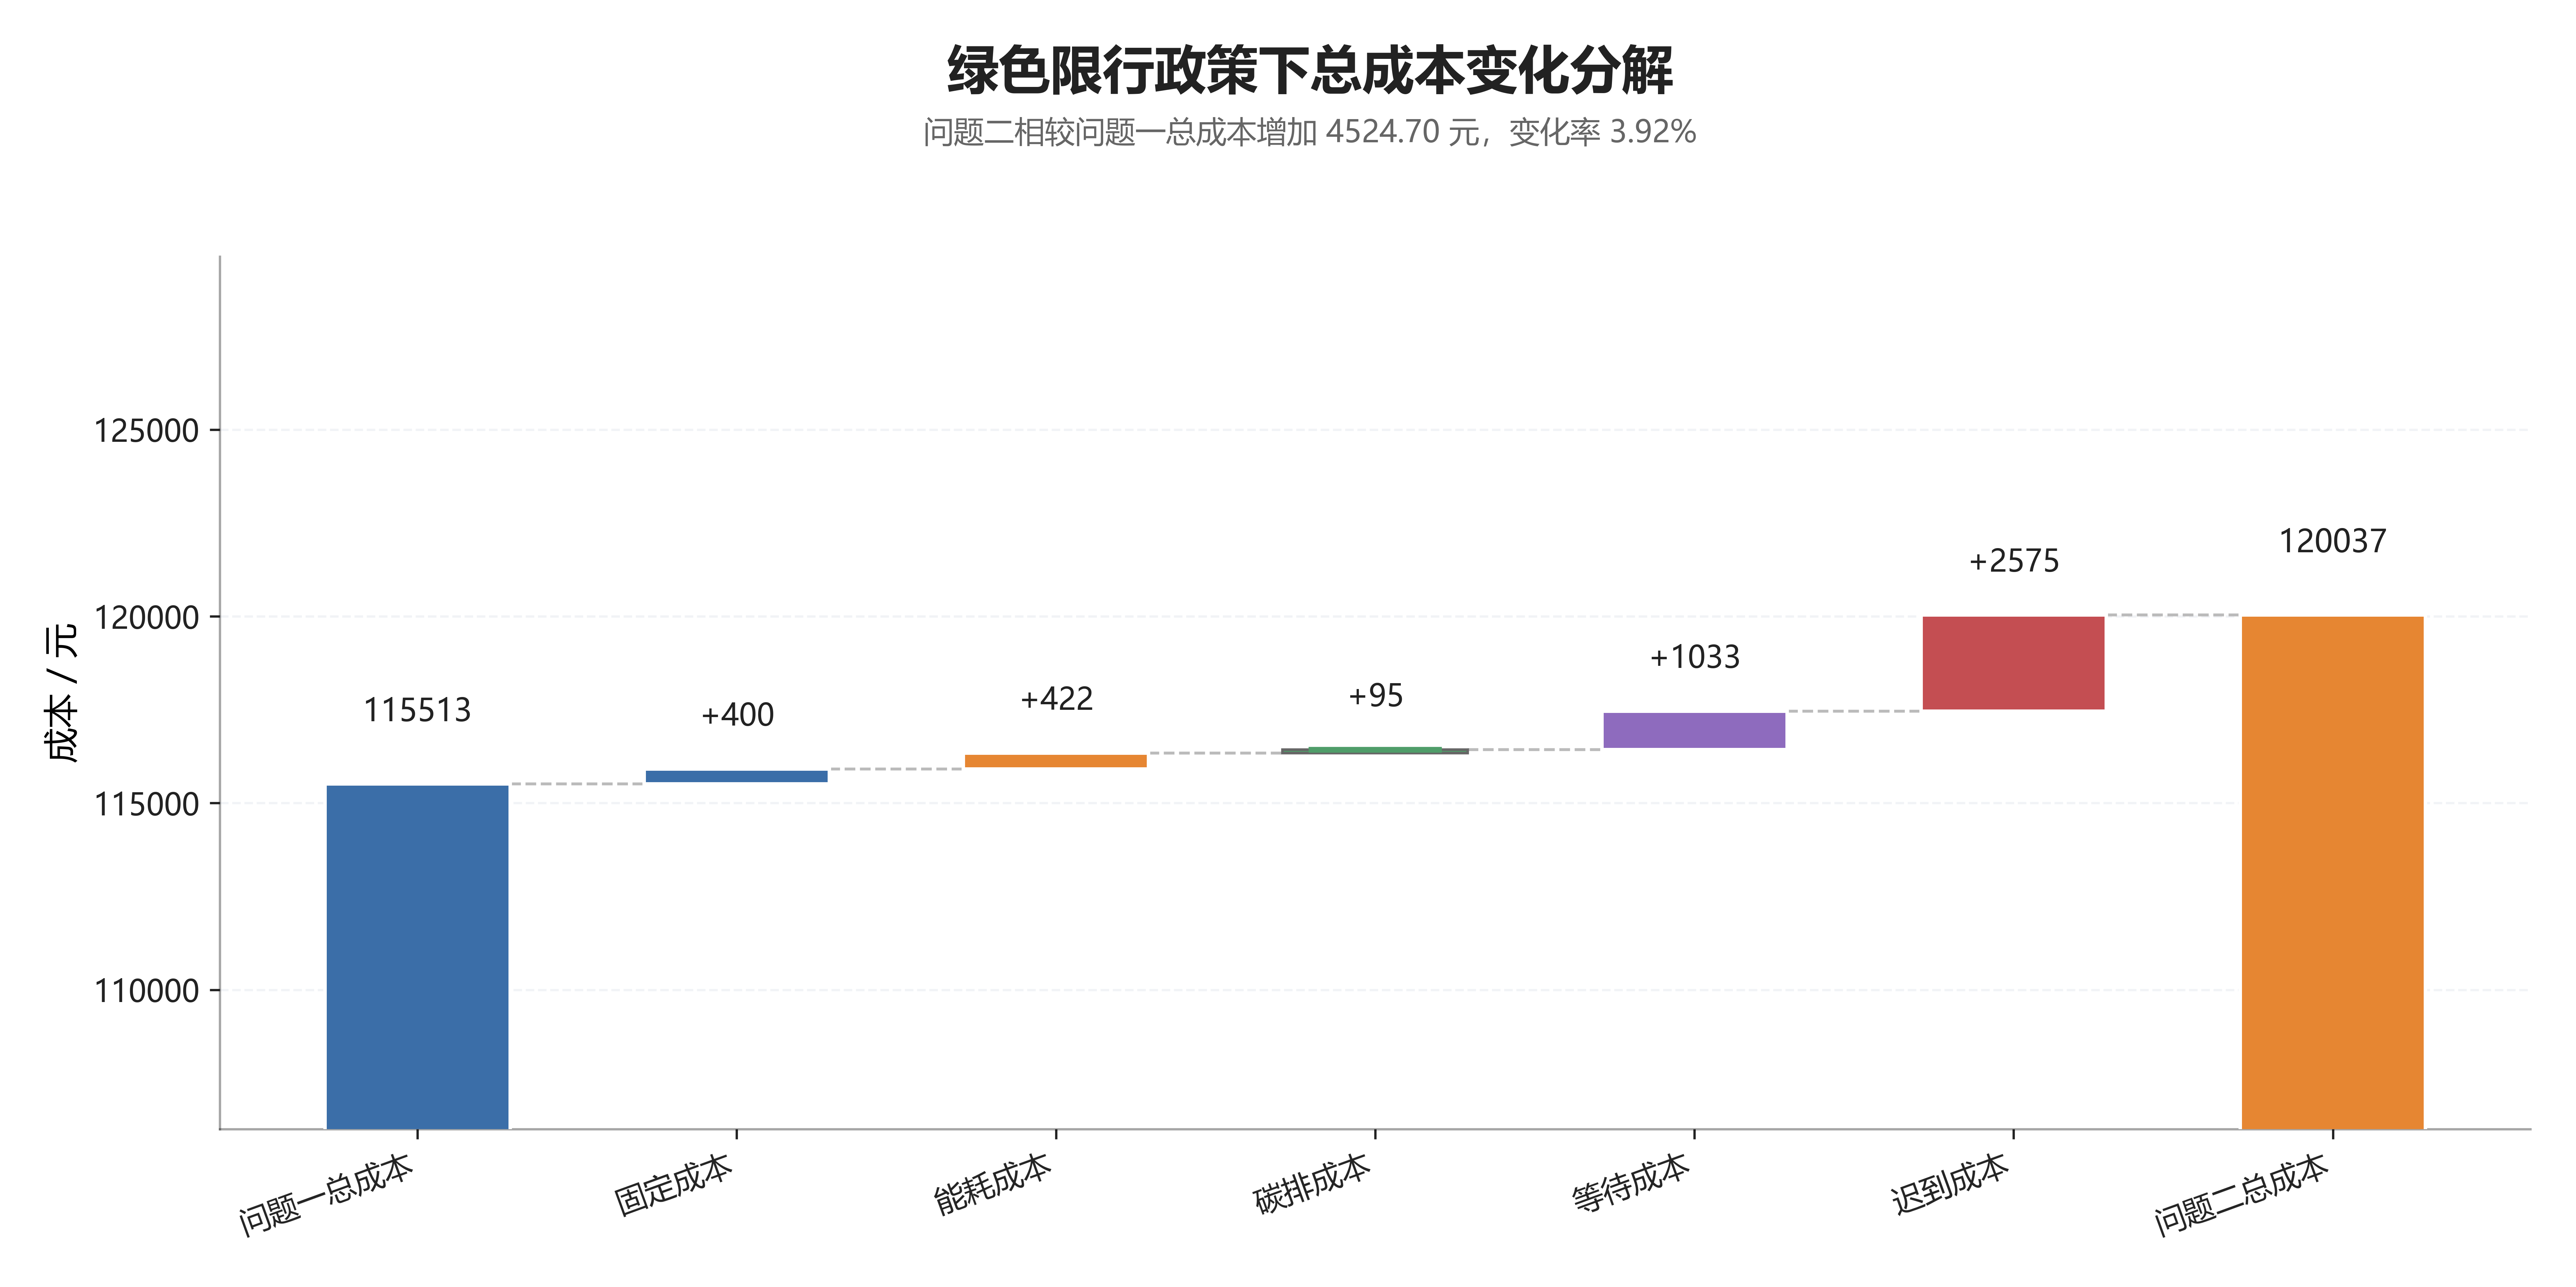
\includegraphics[width=0.85\textwidth]{../figures/paper/p2_cost_waterfall.png}
    \caption{绿色限行政策下总成本变化分解}
    \label{fig:p2_cost_waterfall}
\end{figure}

由图 \ref{fig:p2_cost_waterfall} 可知，问题二成本增量主要来源于时间窗相关成本。其中，迟到成本增加 $2575.23$ 元，等待成本增加 $1032.52$ 元，二者构成总成本增量的主要部分；固定成本、能耗成本和碳排放成本虽有所上升，但增幅相对有限。这表明绿色限行政策对调度结果的影响主要体现在压缩燃油车可服务时段、降低路径时序安排灵活性，而非显著增加行驶距离。

进一步看，迟到成本增量最为明显。其原因在于绿色区任务需优先由新能源车辆承担，或延后至 $16{:}00$ 后由燃油车服务；在新能源运力有限的情况下，部分任务服务时刻被迫后移，进而放大时间窗违约成本。由于问题一迟到成本基数较小，其相对增幅较大，因此更应关注其绝对增量及其反映的时效风险。

从车辆使用结构看，问题一与问题二的车型使用数量对比如图 \ref{fig:p2_vehicle_compare} 所示。

\begin{figure}[H]
    \centering
    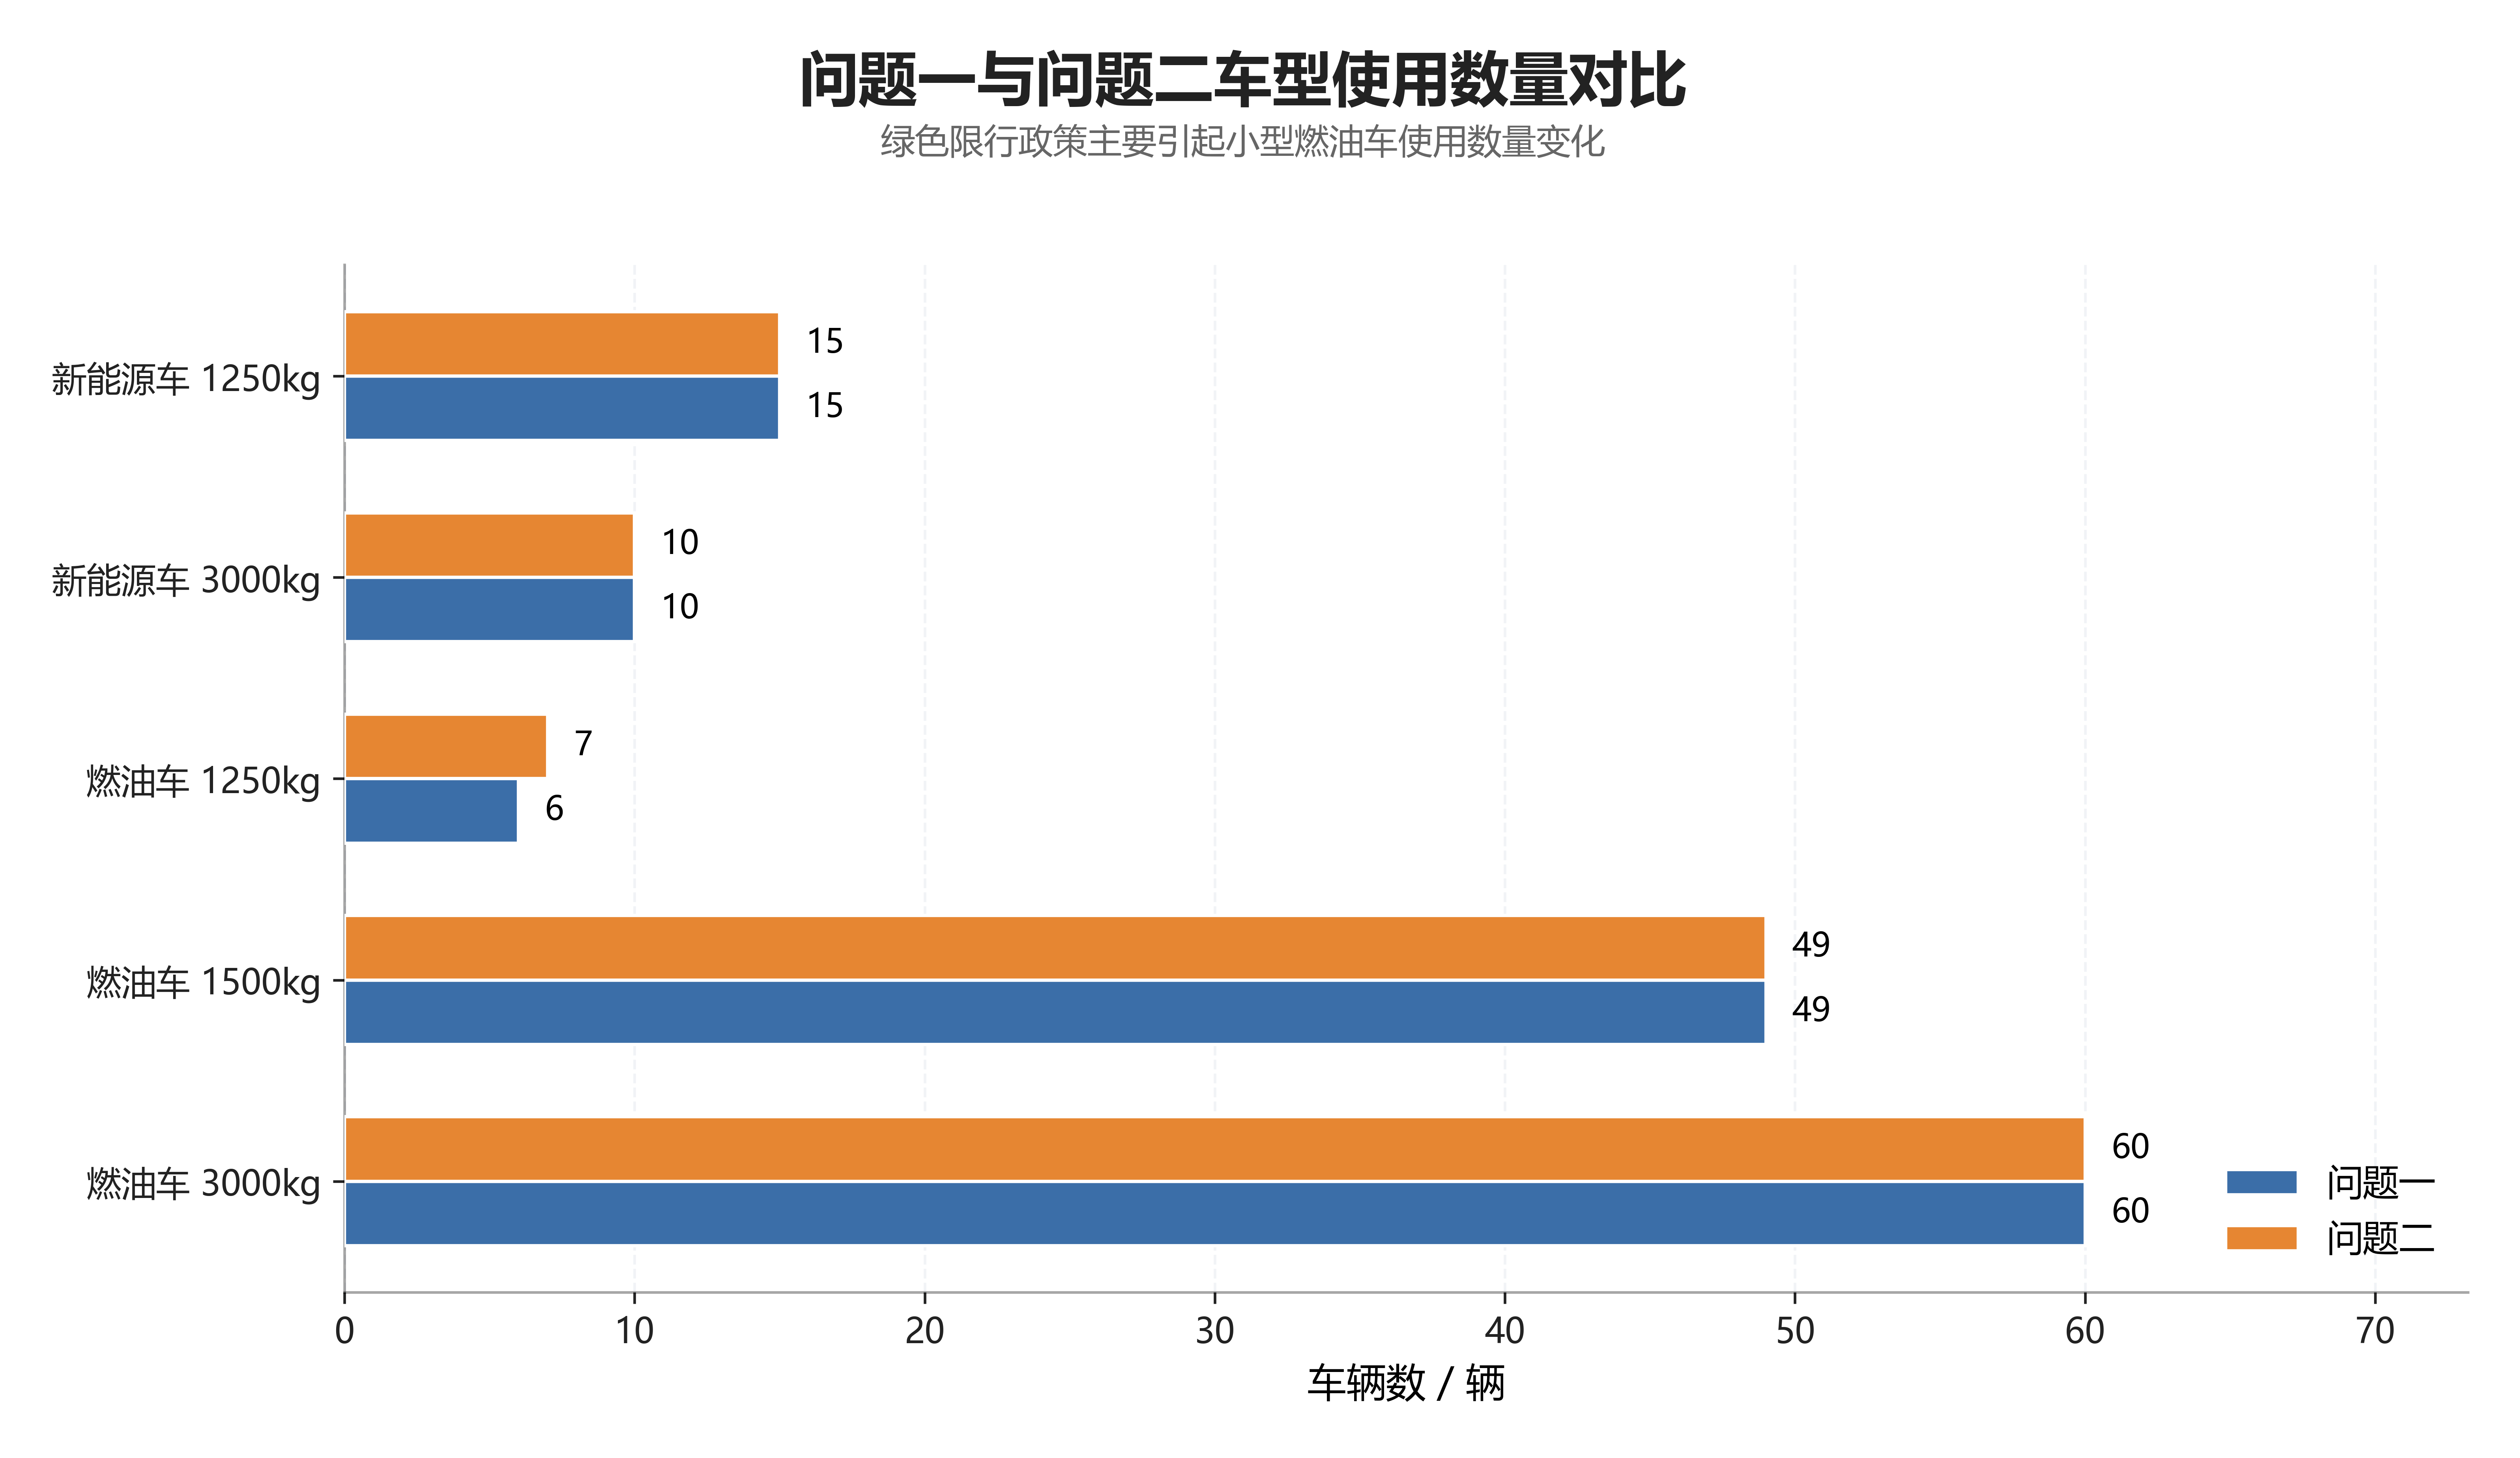
\includegraphics[width=0.85\textwidth]{../figures/paper/p2_cartype.png}
    \caption{问题一与问题二车型使用数量对比}
    \label{fig:p2_vehicle_compare}
\end{figure}

图 \ref{fig:p2_vehicle_compare} 表明，两类新能源车辆在两种情形下均已全部启用，说明新能源运力处于饱和状态。由于新能源车辆无法完全承担绿色区任务，系统仍需依赖燃油车在限行结束后补充服务，并额外启用 $1$ 辆燃油车 $1250\,\mathrm{kg}$ 型车辆，带来 $400$ 元固定成本增量。同时，路径重排使总配送距离略有增加，进而导致能耗成本和碳排放成本小幅上升。

从碳排放结果看，问题二总碳排放量由 $12146.42\,\mathrm{kg}$ 增至 $12292.33\,\mathrm{kg}$，增加 $145.91\,\mathrm{kg}$，增幅为 $1.20\%$。这表明，在现有车队结构下，单纯实施绿色配送区限行并不必然降低企业全局碳排放。该政策能够改善绿色区内车辆通行结构，但当新能源运力不足时，燃油车延后服务和路径重组可能使整体配送距离与总排放量小幅上升。

综上，绿色配送区限行政策能够促进绿色区任务向新能源车辆转移，但在新能源运力不足时，也会压缩调度可行空间，提高时间窗成本和整体运营成本。因此，企业应结合新能源车辆配置、绿色区订单预分组和集中配送时段设计进行协同优化，以降低限行政策带来的额外成本。

%%%%%%%%%%%%%%%%%%%%%%%%%%%%%%%%%%%%%%%%%%%%%%%%%%%%%%%%%%%%% 

\section{问题三：动态事件调度模型建立与求解}

\subsection{问题分析}

问题三在问题二绿色限行方案基础上，研究订单取消、新增订单、配送地址变更和时间窗调整等事件下的路径修复与滚动重优化问题。上述事件会改变剩余任务、服务位置或时间窗约束，属于典型动态车辆路径问题\cite{psaraftis1988,pillac2013}。

动态调度具有实时性和继承性：已完成服务与已执行路径不能回溯修改，完全全局重排又会造成过大扰动。因此，问题三保留原方案主体结构，仅对受扰动的剩余任务进行局部修复。

设动态事件发生时刻为 $\tau$。本文采用“状态冻结--任务更新--局部重优化”策略，冻结已执行部分，更新剩余任务，并在受影响车辆及邻近车辆上用 LNS--VNS 进行路径修复，以兼顾成本优化与方案稳定性。

\begin{figure}[htbp]
  \centering
  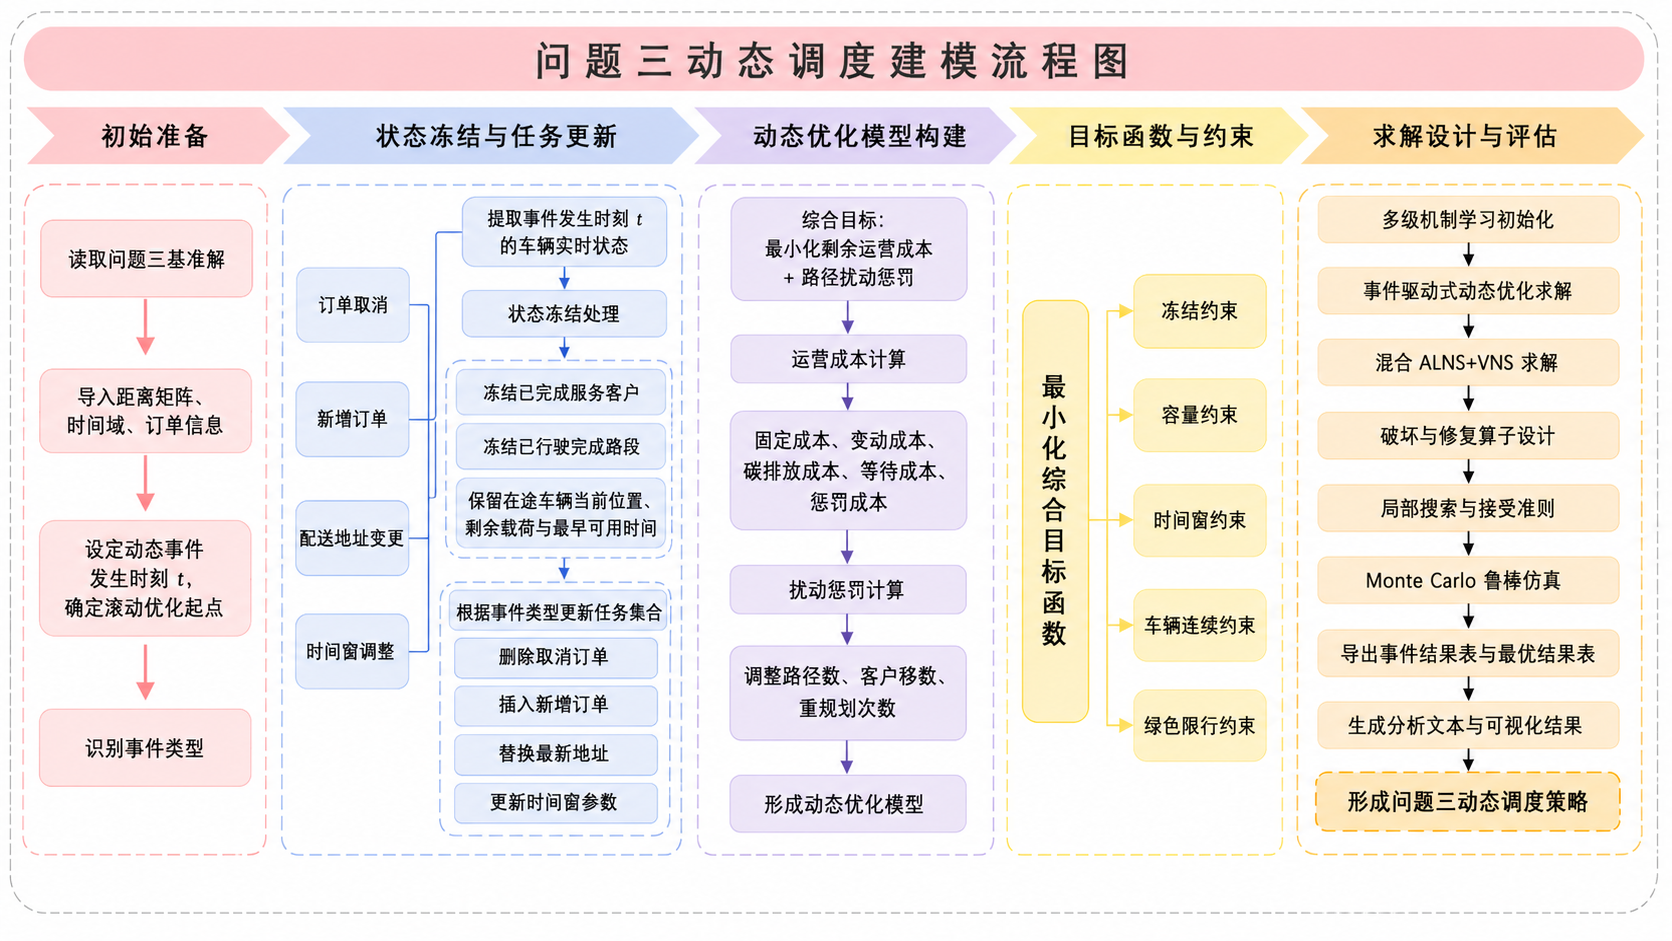
\includegraphics[width = 0.90\textwidth]{../figures/paper/liuchengtu3.png}
  \caption{问题三求解流程图}
  \label{fig:flowchart_q3}
\end{figure}


\subsection{动态调度模型建立}

设动态事件发生时刻为 $\tau$。根据事件发生时车辆和任务的执行状态，将配送任务集合划分为
\begin{equation}
N=N^{done}(\tau)\dot{\cup}N^{lock}(\tau)\dot{\cup}N^{rem}(\tau),
\end{equation}
其中，$N^{done}(\tau)$ 表示事件发生前已经完成服务的任务集合，$N^{lock}(\tau)$ 表示车辆正在服务或正在行驶、短时间内暂不可调整的任务集合，$N^{rem}(\tau)$ 表示尚未服务且仍可重新安排的任务集合，$\dot{\cup}$ 表示集合互不相交。

不同类型动态事件均可转化为剩余任务集合或任务参数的更新：订单取消对应删除相关任务，新增订单对应加入新任务，地址变更对应更新客户位置或替换为新任务，时间窗调整对应修改相关任务的时间窗参数。记事件更新后的剩余任务集合为 $\widetilde{N}^{rem}(\tau)$，新增任务集合为 $N^{new}(\tau)$，则动态待优化任务集合为
\begin{equation}
N^{dyn}(\tau)=\widetilde{N}^{rem}(\tau)\cup N^{new}(\tau).
\end{equation}

为保持已执行方案的稳定性，对已完成任务、已执行弧段和暂不可调整任务实施冻结。设 $\hat{x}_{ijk}$ 和 $\hat{g}_{ik}$ 分别为事件发生前原方案中的路径弧变量和任务分配变量，则有
\begin{equation}
x_{ijk}=\hat{x}_{ijk},\qquad (i,j,k)\in A^{done}(\tau),
\end{equation}
\begin{equation}
g_{ik}=\hat{g}_{ik},\qquad i\in N^{done}(\tau)\cup N^{lock}(\tau),\ k\in K,
\end{equation}
其中，$A^{done}(\tau)$ 表示事件发生前已完成行驶的弧段集合。上述约束使动态调度仅作用于事件后的可调整部分。

对于车辆 $k$，其在事件发生后的最早可重新调度时刻定义为
\begin{equation}
T_k^{ava}(\tau)=
\begin{cases}
\tau, & \text{车辆空闲},\\
\tau+\bar{s}_k(\tau), & \text{车辆正在服务},\\
\tau+\bar{t}_k(\tau), & \text{车辆正在行驶},
\end{cases}
\end{equation}
其中，$\bar{s}_k(\tau)$ 和 $\bar{t}_k(\tau)$ 分别表示车辆 $k$ 在事件时刻的剩余服务时间和剩余行驶时间。滚动优化以 $T_k^{ava}(\tau)$ 时刻的车辆位置、载荷状态和剩余容量作为初始条件，重新安排 $N^{dyn}(\tau)$ 中的可调整任务。

动态调度需同时降低剩余配送成本并控制方案扰动，目标函数设为
\begin{equation}
\min Z^{dyn}
=
C^{dyn}_{oper}
+
\lambda_1\Delta N^{route}
+
\lambda_2\Delta N^{ass}
+
\lambda_3\Delta N^{arc},
\label{eq:dynamic_objective}
\end{equation}
其中，$C^{dyn}_{oper}$ 为事件后剩余任务运营成本，$\Delta N^{route}$、$\Delta N^{ass}$ 和 $\Delta N^{arc}$ 分别为调整路径数、任务改派数和弧段变化数，$\lambda_1,\lambda_2,\lambda_3$ 为对应扰动惩罚系数。

\subsection{事件驱动滚动优化算法}

针对上述动态事件，本文在问题二方案基础上设计事件驱动滚动时域 LNS--VNS 算法。算法以 $\tau$ 为分界点冻结已执行和暂不可调整状态，仅对事件后可调整任务进行局部修复。

设问题二基准路径方案为 $R^0$，事件发生后的动态待优化任务集合为 $N^{dyn}(\tau)$，受影响车辆集合为 $K^{aff}$，邻近车辆集合为 $K^{nei}$。为控制动态调整范围，本文仅选取受影响车辆及其邻近车辆构成局部优化车辆集合：
\begin{equation}
K^{sub}=K^{aff}\cup K^{nei}.
\end{equation}

动态事件统一转化为任务集合或任务属性更新：取消订单删除任务，新增订单加入任务，地址变更等价于“删旧插新”，时间窗调整则修改相应时间窗。

\subsubsection{动态重优化参数设置}

为兼顾响应速度与求解质量，问题三仅在受影响车辆及其邻近车辆构成的局部子问题上进行滚动重优化。算法采用多随机种子独立运行，并在每类动态事件中选取动态目标函数 $Z_{\mathrm{dyn}}$ 最小的方案作为最终重优化结果。主要参数如表 \ref{tab:dynamic_parameters} 所示。

\begin{table}[!htbp]
\centering
\caption{问题三动态重优化与鲁棒性检验参数设置}
\label{tab:dynamic_parameters}
\small
\renewcommand{\arraystretch}{1.20}
\setlength{\tabcolsep}{4pt}
\arrayrulecolor{tableline}

\begin{tabular}{
>{\centering\arraybackslash}p{2.2cm}
>{\raggedright\arraybackslash}p{9.0cm}
>{\centering\arraybackslash}p{3.0cm}}
\toprule
\rowcolor{tablehead}
\textbf{参数} & \centering\textbf{含义} & \textbf{取值} \\
\midrule

$\mathcal{S}^{\mathrm{dyn}}$ 
& 动态重优化随机种子集合 
& $\{1,7,21,42,66\}$ \\

\rowcolor{tablerow}
$\tau$ 
& 动态事件发生时刻，以 $8{:}00$ 为时间零点 
& $180\,\mathrm{min}$，即 $11{:}00$ \\

$I_{\max}^{\mathrm{dyn}}$ 
& 动态重优化最大迭代次数 
& $220$ \\

\rowcolor{tablerow}
$t_{\max}^{\mathrm{dyn}}$ 
& 单个随机种子的运行时间上限 
& $35\,\mathrm{s}$ \\

$T_0^{\mathrm{dyn}}$ 
& 模拟退火初始温度 
& $1800$ \\

\rowcolor{tablerow}
$\alpha^{\mathrm{dyn}}$ 
& 模拟退火降温系数 
& $0.988$ \\

$p^{\mathrm{dyn}}$ 
& 每次破坏操作移除的任务比例 
& $[0.08,0.25]$ \\

\rowcolor{tablerow}
$N_{\mathrm{nei}}$ 
& 动态事件中选取的邻近路径数量 
& $6$ \\

$N_{\mathrm{reloc}}$ 
& VNS 中 relocate 候选任务上限 
& $24$ \\

\rowcolor{tablerow}
$N_{\mathrm{swap}}$ 
& VNS 中 swap 随机交换次数上限 
& $30$ \\

$N_{\mathrm{2opt}}$ 
& VNS 中单路径 2-opt 尝试次数上限 
& $16$ \\

\rowcolor{tablerow}
$N_{\mathrm{MC}}$ 
& Monte Carlo 速度扰动仿真次数 
& $50$ \\

\bottomrule
\end{tabular}

\arrayrulecolor{black}
\end{table}

局部子问题采用 LNS--VNS 混合搜索：LNS 调整可变任务的车辆分配和访问顺序，VNS 通过 relocate、swap 和 2-opt 邻域改进候选路径\cite{mladenovic1997}，并用模拟退火准则接受候选解\cite{kirkpatrick1983}。流程见算法 \ref{alg:dynamic_lns_vns}。

\begin{algorithm}[!htbp]
\caption{事件驱动滚动时域 LNS--VNS 动态调度算法}
\label{alg:dynamic_lns_vns}
\small
\begin{algorithmic}[1]
\Require 基准调度方案 $R^0$，动态事件 $e$，事件时刻 $\tau$，
随机种子集合 $\mathcal{S}^{\mathrm{dyn}}$，最大迭代次数 $I_{\max}$，
初始温度 $T_0$，降温系数 $\alpha$
\Ensure 动态重优化方案 $R^{*}$

\State $(N^{done},N^{lock},N^{rem})\gets \textsc{Partition}(R^0,\tau)$；
\State 冻结已完成任务、暂不可调整任务、车辆状态及已执行弧段；
\State $N^{dyn}\gets \textsc{UpdateTasks}(N^{rem},e)$；
\State 识别 $K^{aff}$ 和 $K^{nei}$，令 $K^{sub}\gets K^{aff}\cup K^{nei}$；
\State $R^{init}\gets \textsc{BuildInitial}(R^0,N^{dyn},K^{sub})$；
\State $R^{*}\gets R^{init}$，$Z^{*}\gets Z_{\mathrm{dyn}}(R^{init})$；

\For{$s\in\mathcal{S}^{\mathrm{dyn}}$}
    \State 设置随机种子 $s$；
    \State $R^{cur}\gets R^{init}$，$R^{best}\gets R^{init}$，$T\gets T_0$；

    \For{$iter=1$ \textbf{to} $I_{\max}$}
        \State 对 $K^{sub}$ 内可调整任务执行 LNS 破坏操作，得到 $R^d$；
        \State 采用修复算子重插入被移除任务，得到 $R^r$；
        \State 对 $R^r$ 执行 VNS 局部搜索，生成候选解 $R'$；
        \State 检验 $R'$ 的容量、时间窗、绿色限行和冻结约束；

        \If{$R'$ 可行}
            \State $\Delta Z\gets Z_{\mathrm{dyn}}(R')-Z_{\mathrm{dyn}}(R^{cur})$；
            \If{$\Delta Z<0$ \textbf{or} $u<\exp(-\Delta Z/T),\ u\sim U(0,1)$}
                \State $R^{cur}\gets R'$；
            \EndIf
            \If{$Z_{\mathrm{dyn}}(R^{cur})<Z_{\mathrm{dyn}}(R^{best})$}
                \State $R^{best}\gets R^{cur}$；
            \EndIf
        \EndIf

        \State $T\gets \alpha T$；
    \EndFor

    \If{$Z_{\mathrm{dyn}}(R^{best})<Z^{*}$}
        \State $R^{*}\gets R^{best}$，$Z^{*}\gets Z_{\mathrm{dyn}}(R^{best})$；
    \EndIf
\EndFor

\State \Return $R^{*}$；
\end{algorithmic}
\end{algorithm}

LNS 阶段采用随机移除、高成本任务移除和相关任务移除三类破坏算子，分别用于增强扰动、优先调整高成本任务和成组重构相近任务。修复阶段采用最小增量插入、regret-2 插入、regret-3 插入和低扰动插入，其中低扰动插入优先保留原任务--车辆匹配和局部访问顺序。

VNS 阶段采用 relocate、swap 和 2-opt 三类邻域算子，分别从任务重定位、路径间交换和路径内顺序优化三个层面改进候选解。

每类动态事件均按表 \ref{tab:dynamic_parameters} 中的参数独立运行，并选取动态目标函数 $Z_{\mathrm{dyn}}$ 最小的方案作为最终重优化结果。获得 $R^{*}$ 后，本文按题目给定速度分布进行 Monte Carlo 扰动仿真，检验随机交通条件下的鲁棒性。


为控制对原配送计划的扰动，动态目标函数引入调整路径数、任务改派数和弧段变化数三类惩罚项，系数见表 \ref{tab:disturbance_parameters}。

\begin{table}[H]
\centering
\caption{动态调度扰动惩罚系数设置}
\label{tab:disturbance_parameters}
\small
\renewcommand{\arraystretch}{1.20}
\setlength{\tabcolsep}{4pt}
\arrayrulecolor{tableline}

\begin{tabular}{
>{\centering\arraybackslash}p{2.2cm}
>{\raggedright\arraybackslash}p{9.2cm}
>{\centering\arraybackslash}p{3.0cm}}
\toprule
\rowcolor{tablehead}
\textbf{参数} & \centering\textbf{含义} & \textbf{取值} \\
\midrule

$\lambda_1$ 
& 调整路径数惩罚系数 
& $120$ \\

\rowcolor{tablerow}
$\lambda_2$ 
& 任务改派惩罚系数 
& $35$ \\

$\lambda_3$ 
& 弧段扰动惩罚系数 
& $8$ \\

\rowcolor{tablerow}
$\lambda_4$ 
& 容量不可行惩罚系数，用于候选解筛选与搜索引导 
& $10000$ \\

\bottomrule
\end{tabular}

\arrayrulecolor{black}
\end{table}

与式 \eqref{eq:dynamic_objective} 一致，本文扰动惩罚系数取
\begin{equation}
(\lambda_1,\lambda_2,\lambda_3)=(120,35,8).
\end{equation}

需要说明的是，$\lambda_4$ 仅用于搜索过程中对容量不可行候选解施加大惩罚，以引导算法回到可行区域；最终输出方案必须满足容量约束，因此 $\lambda_4$ 不计入最终动态目标函数。

上述参数下，LNS--VNS 通过破坏--修复和邻域改进生成方案；多随机种子、模拟退火和扰动惩罚共同兼顾求解质量与方案稳定性。

\subsection{动态事件案例设置与求解结果}

问题二总成本对应完整配送周期，问题三仅评价事件后剩余任务，二者统计范围不同。本文因此以 $\tau$ 之后仍需执行的任务为评价对象，事件前已完成服务和不可调整车辆状态均视为历史既定部分。

设问题二原方案在事件发生后继续执行剩余任务的成本为动态评估基准成本 $Z_0^{\mathrm{dyn}}$，事件初始响应方案成本为 $Z_{\mathrm{init}}^{\mathrm{dyn}}$，滚动重优化后成本为 $Z_*^{\mathrm{dyn}}$。定义
\begin{equation}
\Delta C_{\mathrm{save}}
=
Z_{\mathrm{init}}^{\mathrm{dyn}}-Z_*^{\mathrm{dyn}},
\qquad
\Delta C_{\mathrm{base}}
=
Z_*^{\mathrm{dyn}}-Z_0^{\mathrm{dyn}}.
\end{equation}
其中，$\Delta C_{\mathrm{save}}$ 为重优化相对初始响应方案的节约成本，$\Delta C_{\mathrm{base}}$ 为相对动态评估基准的成本变化；$\Delta C_{\mathrm{base}}<0$ 仅表示剩余路径局部结构得到改进。

四类事件均设定在 $11{:}00$ 发生，即 $\tau=180\,\mathrm{min}$。以问题二最终调度方案作为动态响应基准，冻结事件发生前已完成服务及暂不可调整车辆状态后，重新计算事件发生后剩余任务的运营成本，得动态评估基准成本 $Z_0^{\mathrm{dyn}}=110423.11$ 元。问题二完整方案的总配送距离为 $18632.96\,\mathrm{km}$，该距离仅用于说明基准方案的整体路径规模，不与问题三剩余任务成本直接比较。

本文在问题二基准调度方案基础上，构造四类相互独立的典型动态事件：

\begin{itemize}
    \item {\heiti E1：订单取消。} 尚未服务的任务 $92\_1$ 被取消，系统删除该任务，并对其所在路径及邻近路径进行局部重优化；
    \item {\heiti E2：新增订单。} 客户 $52$ 临时产生新增配送任务 $NEW\_52$，系统将其插入剩余待服务任务集合，并重新优化相关路径；
    \item {\heiti E3：配送地址变更。} 任务 $36\_2$ 的配送地址由客户 $36$ 变更为客户 $64$，等价处理为删除原任务并插入新任务 $ADDR\_36\_TO\_64$；
    \item {\heiti E4：时间窗收紧。} 任务 $7\_1$ 与 $50\_4$ 的最晚服务时间临时提前，系统重新调整相关任务访问顺序和车辆分配。
\end{itemize}

针对四类事件，本文先更新剩余任务并生成初始响应方案，再对受影响车辆及邻近车辆调用多随机种子 LNS--VNS 重优化。结果见表 \ref{tab:p3_event_result}。

\begin{table}[H]
\centering
\caption{问题三动态事件重优化结果}
\label{tab:p3_event_result}
\small
\renewcommand{\arraystretch}{1.18}
\setlength{\tabcolsep}{5pt}
\arrayrulecolor{tableline}
\resizebox{0.98\textwidth}{!}{
\begin{tabular}{c c r r r r c c}
\toprule
\rowcolor{tablehead}
\textbf{事件} & \textbf{类型} & \textbf{初始成本/元} & \textbf{重优化成本/元} & \textbf{节约成本/元} & \textbf{较动态基准变化/元} & \textbf{调整路径数} & \textbf{最优随机种子} \\
\midrule
E1 & 订单取消 & 110425.40 & 107304.51 & 3120.89 & -3118.60 & 6 & 7 \\
\rowcolor{tablerow}
E2 & 新增订单 & 110691.53 & 108187.10 & 2504.43 & -2236.01 & 4 & 66 \\
E3 & 地址变更 & 110370.75 & 107400.09 & 2970.66 & -3023.02 & 6 & 7 \\
\rowcolor{tablerow}
E4 & 时间窗收紧 & 110523.60 & 107038.68 & 3484.92 & -3384.42 & 6 & 66 \\
\bottomrule
\end{tabular}
}
\arrayrulecolor{black}
\end{table}

为直观比较事件初始响应方案与滚动重优化方案的成本差异，本文绘制动态事件下的成本对比图，如图 \ref{fig:p3_event_cost_compare} 所示。

\begin{figure}[!htbp]
    \centering
    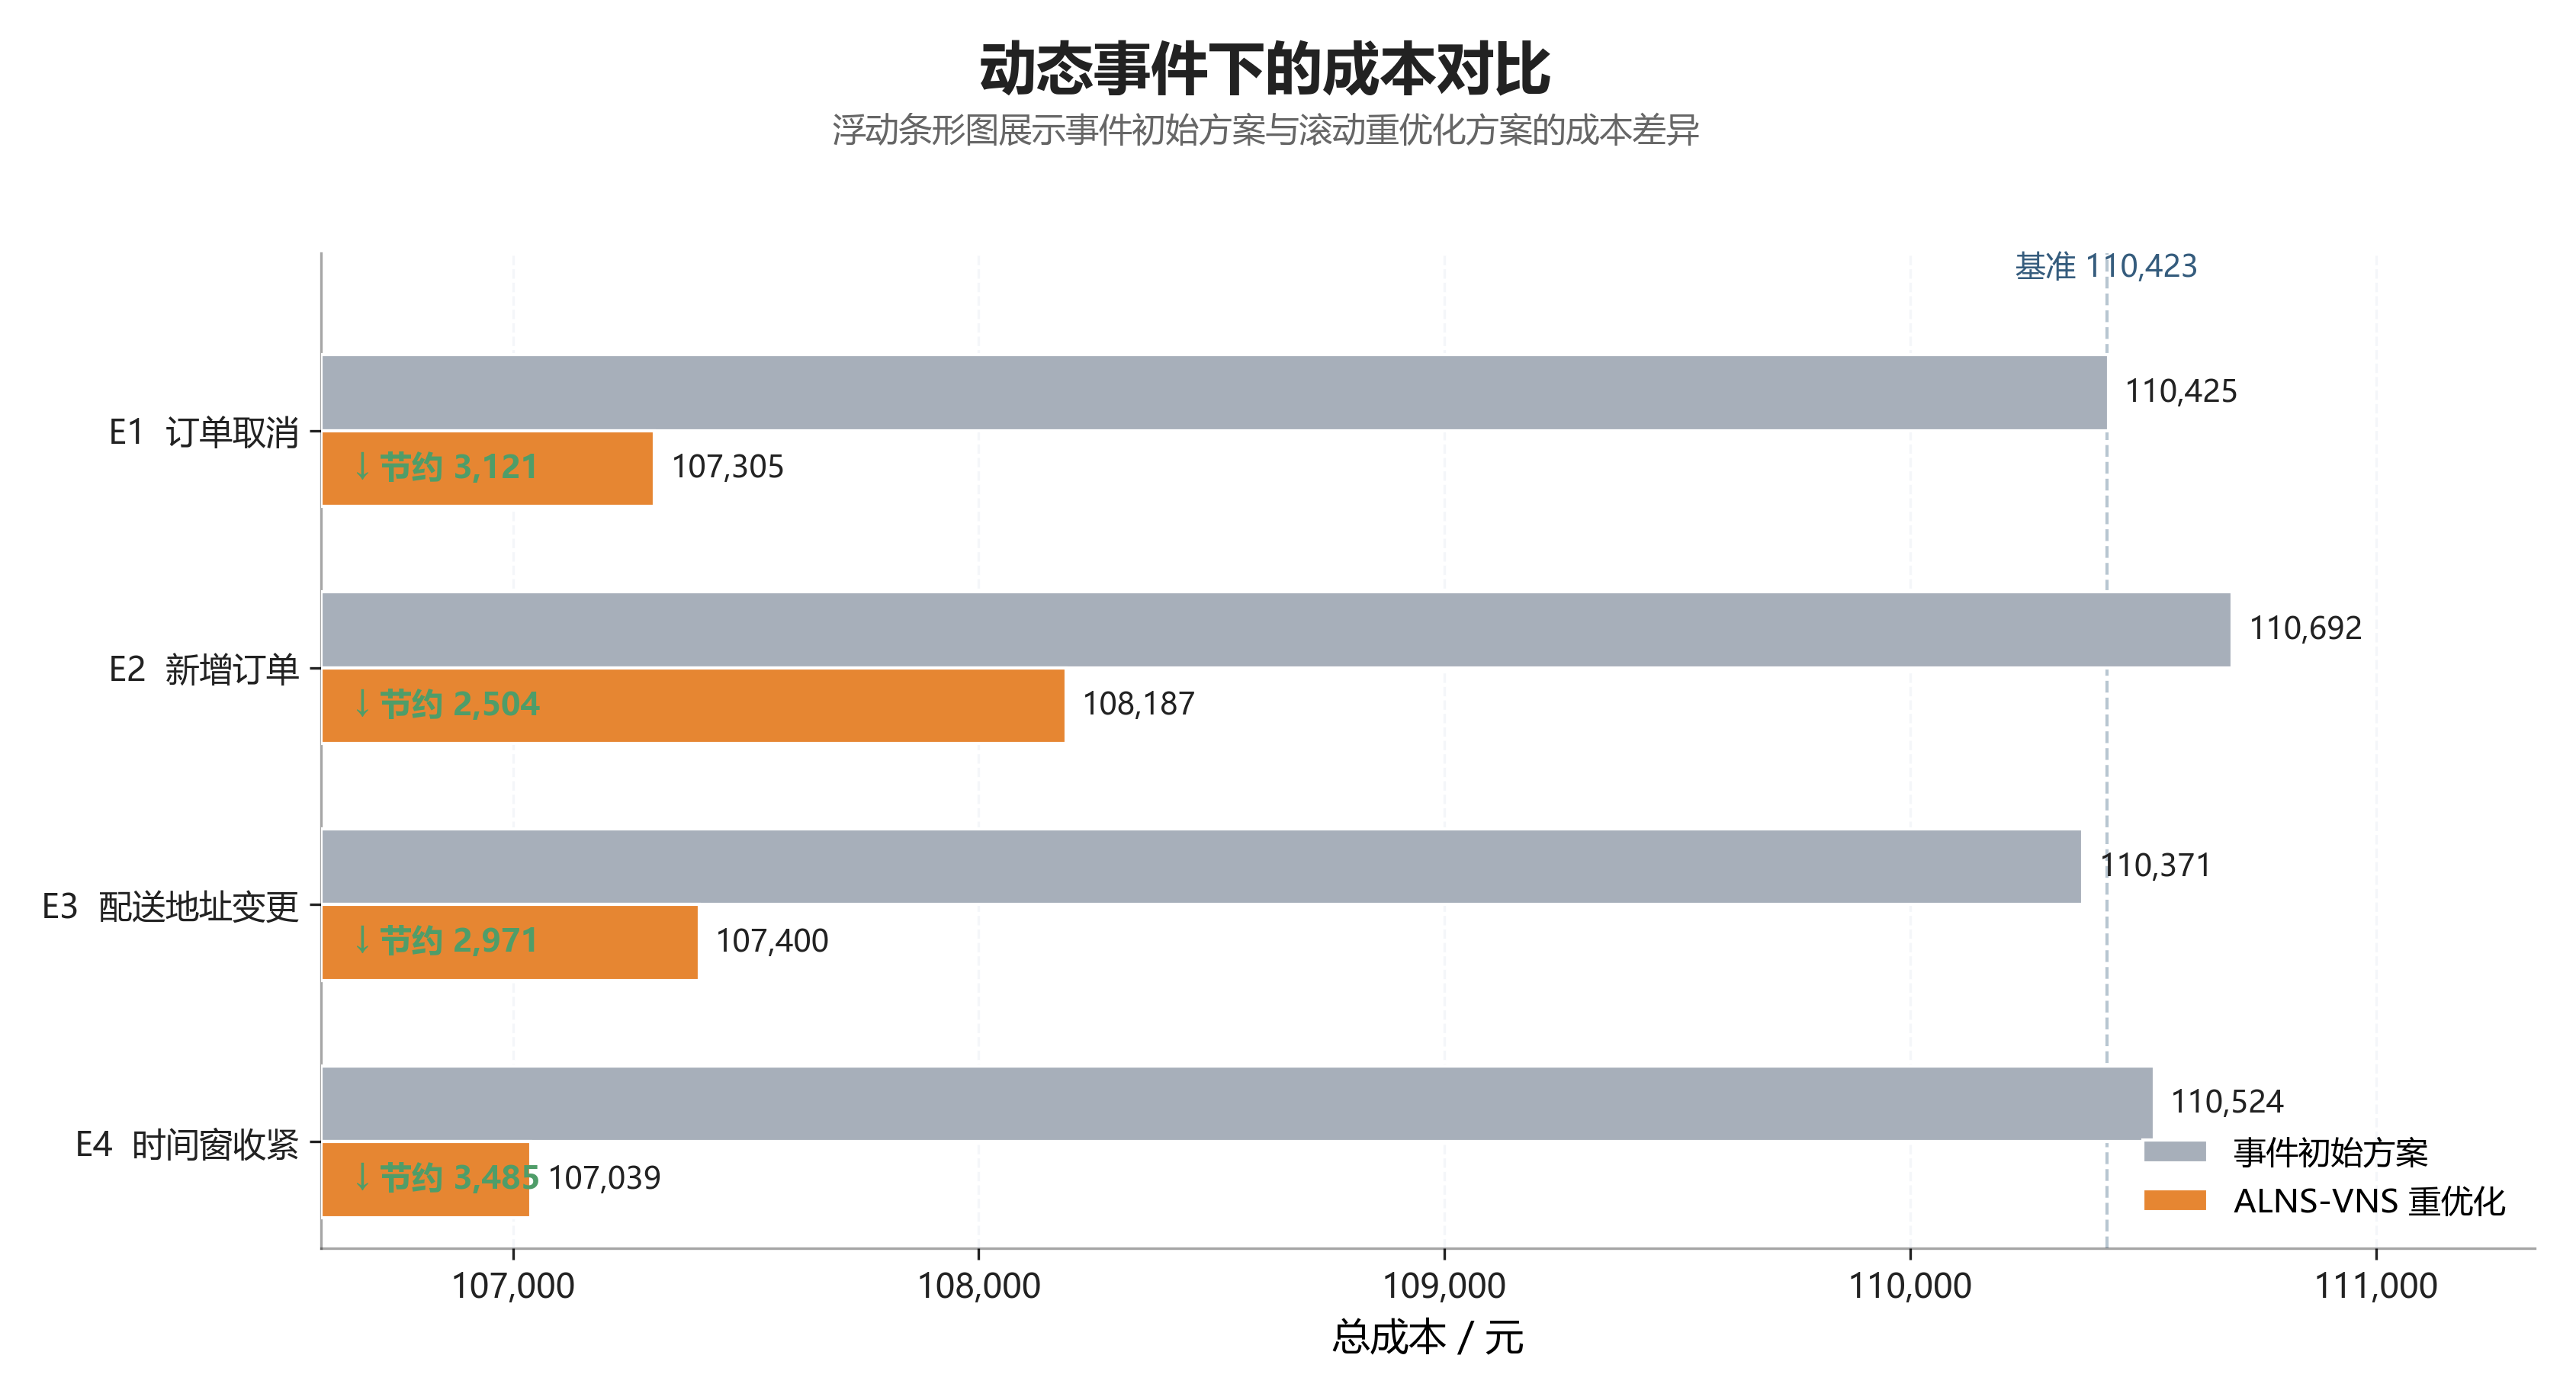
\includegraphics[width=0.78\textwidth]{../figures/paper/p3_cost.png}
    \caption{动态事件下初始响应方案与重优化方案成本对比}
    \label{fig:p3_event_cost_compare}
\end{figure}

由表 \ref{tab:p3_event_result} 和图 \ref{fig:p3_event_cost_compare} 可知，四类事件重优化后均节约成本，金额为 $2504.43$--$3484.92$ 元；其中 E4 节约最多，E2 相对较少。重优化成本均低于 $Z_0^{\mathrm{dyn}}$，说明算法修正了剩余路径中的局部非最优结构。

\subsection{结果分析}

不同事件的影响机制不同：E4 压缩时间窗，时序冲击最强，节约 $3484.92$ 元；E1 取消订单释放服务时间和容量，节约 $3120.89$ 元；E3 地址变更改变局部空间连接，节约 $2970.66$ 元；E2 新增订单增加配送负担，但经局部重构仍节约 $2504.43$ 元。

为评价方案扰动程度，本文统计调整路径数、改派任务数和弧段扰动数，结果见表 \ref{tab:p3_disturbance}。

\begin{table}[H]
\centering
\caption{动态事件路径扰动统计}
\label{tab:p3_disturbance}
\small
\renewcommand{\arraystretch}{1.18}
\setlength{\tabcolsep}{10pt}
\arrayrulecolor{tableline}

\begin{tabular}{c c c c c}
\toprule
\rowcolor{tablehead}
\textbf{事件} & \textbf{类型} & \textbf{调整路径数} & \textbf{改派任务数} & \textbf{弧段扰动数} \\
\midrule
E1 & 订单取消 & 6 & 7 & 25 \\
\rowcolor{tablerow}
E2 & 新增订单 & 4 & 6 & 20 \\
E3 & 地址变更 & 6 & 4 & 18 \\
\rowcolor{tablerow}
E4 & 时间窗收紧 & 6 & 9 & 30 \\
\bottomrule
\end{tabular}

\arrayrulecolor{black}
\end{table}

由表 \ref{tab:p3_disturbance} 可知，四类事件调整路径数均为 $4$--$6$ 条，说明重优化主要围绕受影响车辆及邻近车辆展开。E2 仅调整 $4$ 条路径，扰动最小；E4 改派任务数和弧段扰动数最高，分别为 $9$ 个和 $30$ 个。总体看，该策略能在降低剩余运营成本的同时控制调整幅度。

多随机种子结果显示，E1、E3 的最优种子为 $7$，E2、E4 为 $66$，说明独立多次运行并择优输出有助于降低随机性影响。

为考察随机交通下的稳定性，本文按题目给定分时段车速分布进行
$N_{\mathrm{MC}}=50$ 次 Monte Carlo 仿真，并重新计算行驶时间与成本，
结果如图 \ref{fig:p3_rate} 所示。

\begin{figure}[H]
    \centering
    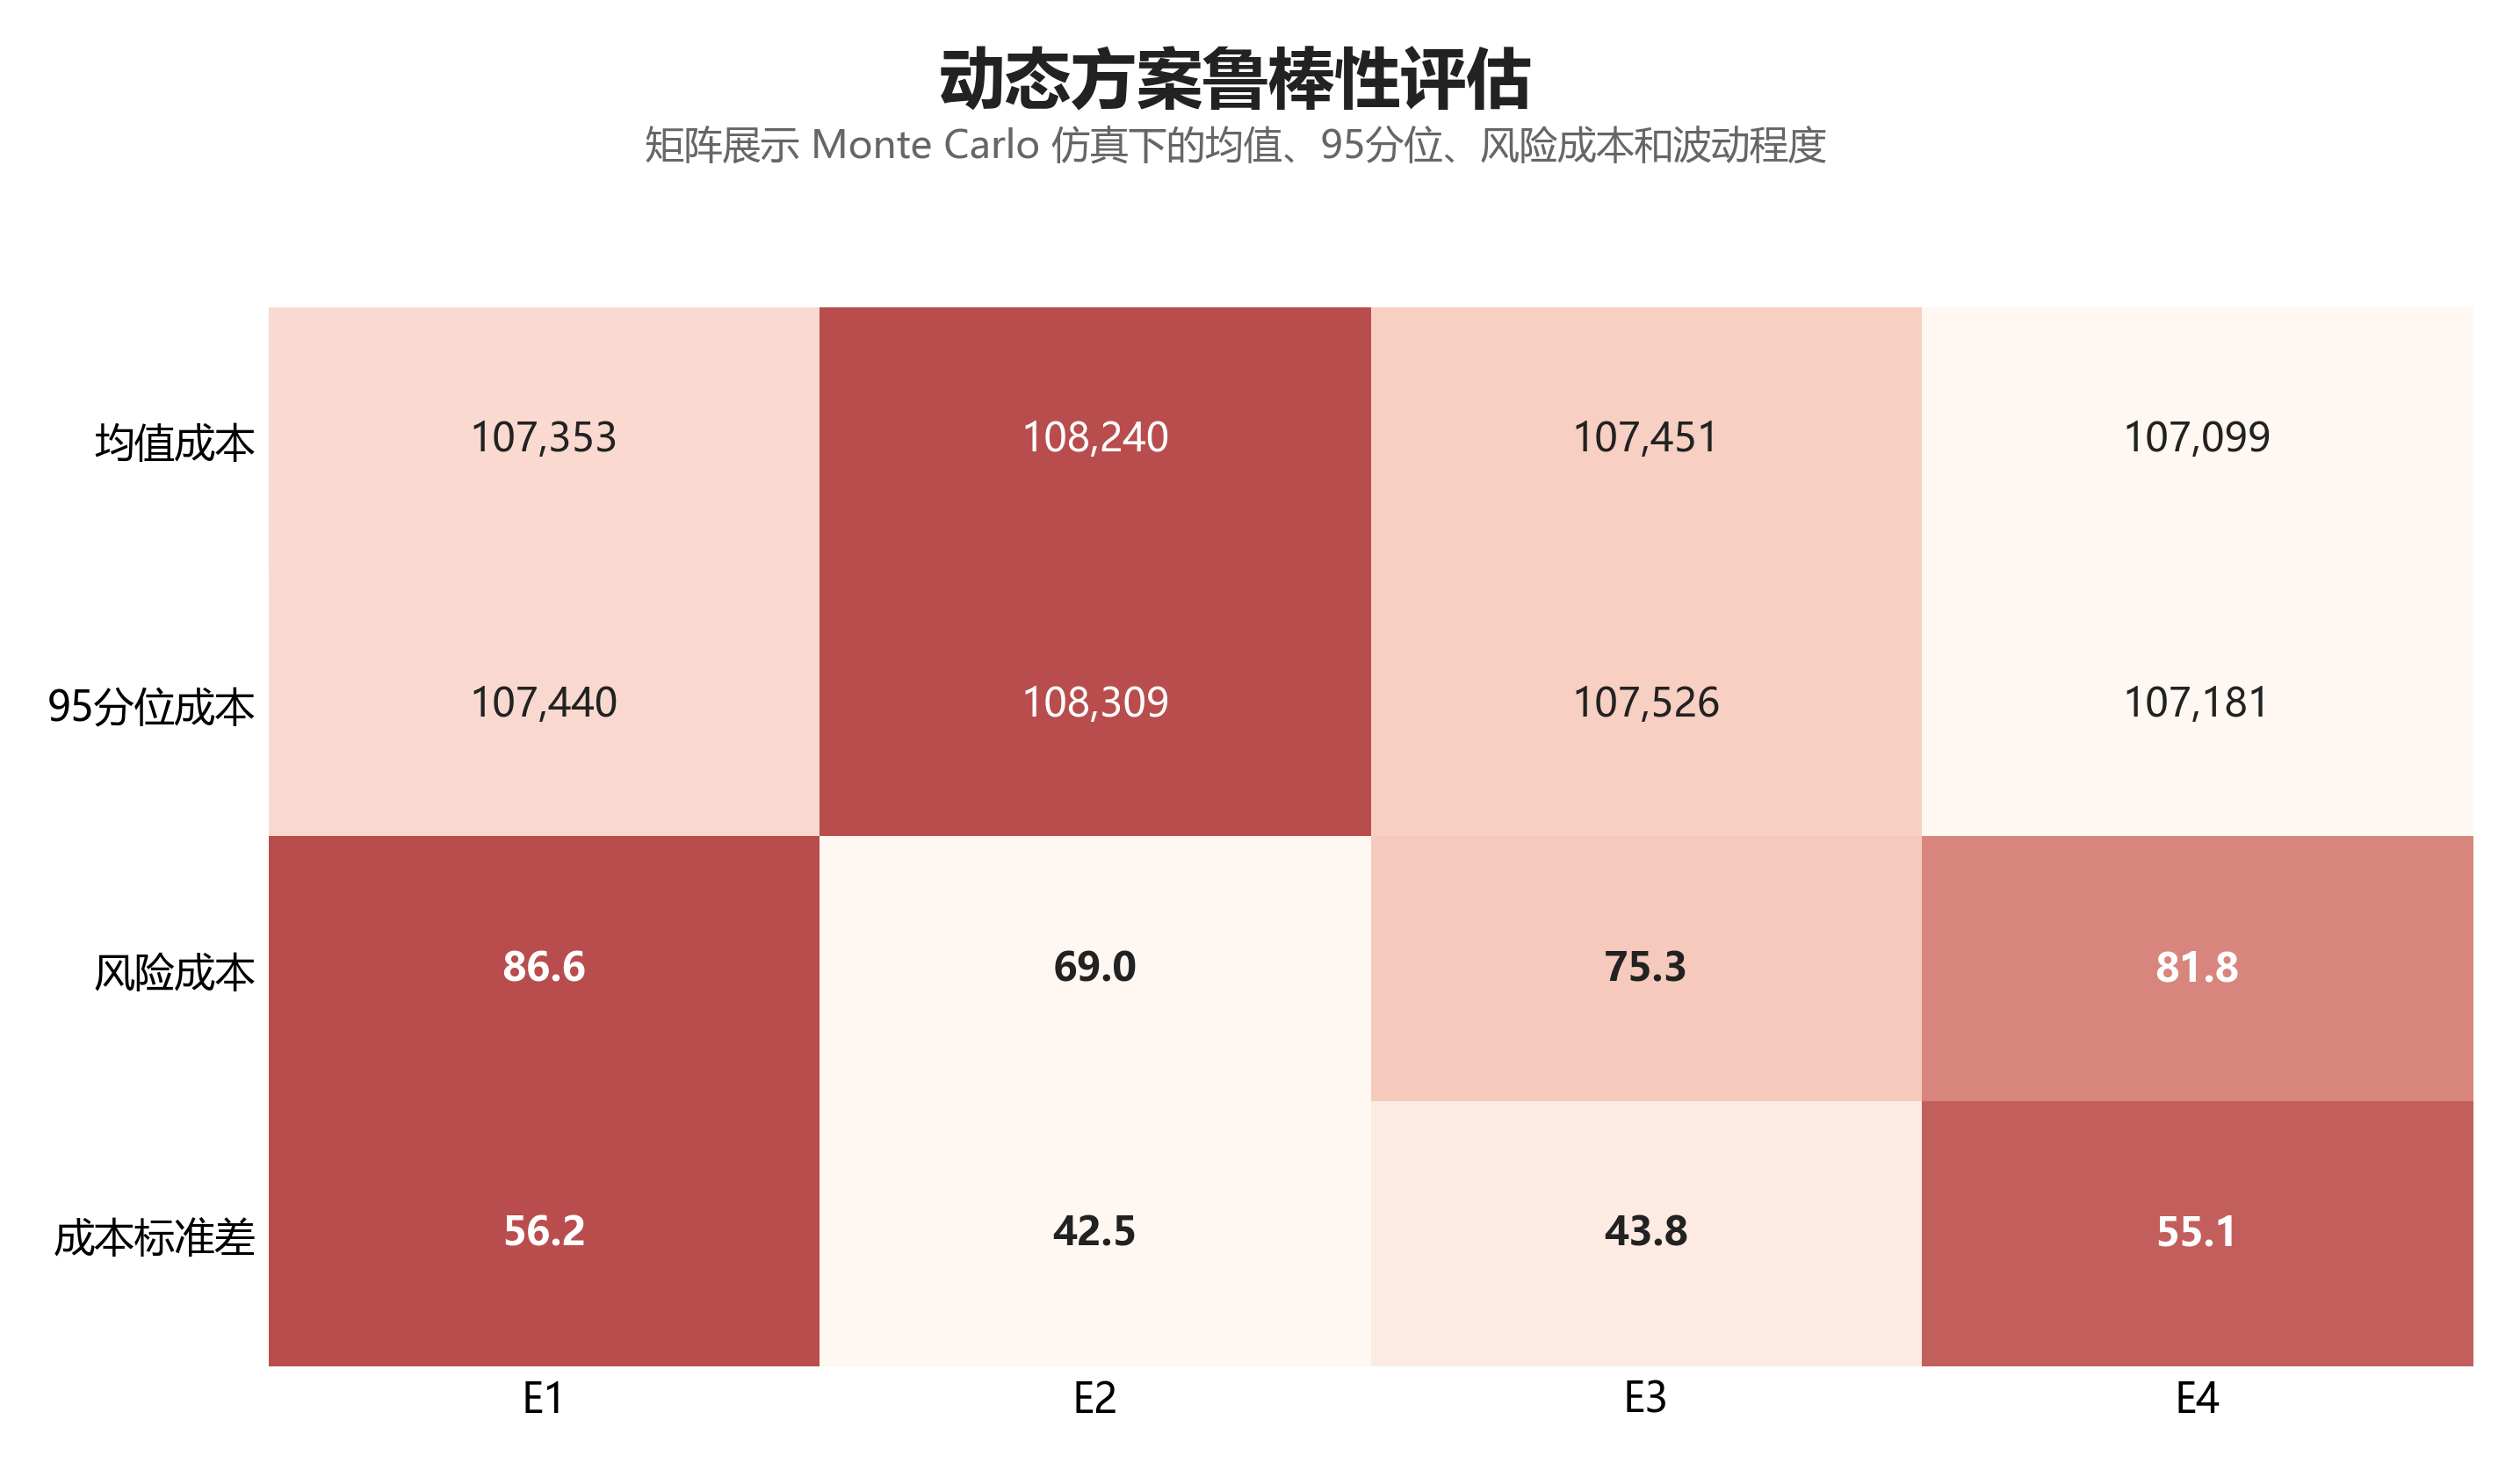
\includegraphics[width=0.75\textwidth]{../figures/paper/p3_rate.png}
    \caption{动态事件重优化方案的鲁棒性评估结果}
    \label{fig:p3_rate}
\end{figure}

由图 \ref{fig:p3_rate} 可知，四类事件的鲁棒均值成本与确定性成本偏差较小，
成本标准差均低于 $60$ 元，风险成本为 $69.00$--$86.64$ 元，
说明方案对车速随机波动具有较好稳定性。

综合来看，初始响应方案用于恢复可行性，LNS--VNS 重优化进一步重组受影响路径。
所提滚动优化策略能处理四类典型扰动，并兼顾成本控制、方案稳定性与实时响应能力。

\FloatBarrier

%%%%%%%%%%%%%%%%%%%%%%%%%%%%%%%%%%%%%%%%%%%%%%%%%%%%%%%%%%%%%

\section{模型的优缺点分析}

\subsection{模型的优点}

\begin{enumerate}
    \item {\heiti\bfseries 三问衔接自然：}
    本文以统一的任务集合、车辆集合、成本口径和约束体系贯穿三个问题，使静态调度、绿色限行和动态响应能够逐层展开。

    \item {\heiti\bfseries 约束刻画较完整：}
    模型综合考虑异质车队、双容量约束、软时间窗、时变车速、能耗、碳排放和绿色配送区限行政策，较好贴合城市配送实际场景。

    \item {\heiti\bfseries 成本评价较细致：}
    路径评估器统一计算固定成本、能耗成本、碳排放成本、等待成本和迟到惩罚成本，并结合车速和载荷变化逐弧评估行驶成本。

    \item {\heiti\bfseries 算法具有可执行性：}
    静态与绿色限行情形采用多随机种子 ALNS 求解，动态事件采用 LNS--VNS 局部重优化，兼顾了成本优化和路径扰动控制。
\end{enumerate}

\subsection{模型的不足}

\begin{enumerate}
    \item {\heiti\bfseries 交通随机性处理仍有简化：}
    主模型采用各时段速度期望值计算行驶时间，随机交通扰动主要用于鲁棒性检验，尚未直接嵌入优化过程。

    \item {\heiti\bfseries 绿色区限行刻画受数据限制：}
    由于题目未提供完整道路网络，本文以车辆到达绿色区任务对应客户点的时刻近似表示入区时刻，与真实边界穿越时刻可能存在偏差。

    \item {\heiti\bfseries 启发式算法难以保证全局最优：}
    ALNS 和 LNS--VNS 能在较短时间内获得高质量可行解，但结果仍受初始解、邻域算子和随机种子影响。
\end{enumerate}

%%%%%%%%%%%%%%%%%%%%%%%%%%%%%%%%%%%%%%%%%%%%%%%%%%%%%%%%%%%%%
%% 参考文献
\section*{参考文献}

\begin{thebibliography}{99}

\bibitem{dantzig1959}
Dantzig G B, Ramser J H. The truck dispatching problem[J]. Management Science, 1959, 6(1): 80-91.

\bibitem{lin2014}
Lin C, Choy K L, Ho G T S, Chung S H, Lam H Y. Survey of green vehicle routing problem: Past and future trends[J]. Expert Systems with Applications, 2014, 41(4): 1118-1138.

\bibitem{solomon1987}
Solomon M M. Algorithms for the vehicle routing and scheduling problems with time window constraints[J]. Operations Research, 1987, 35(2): 254-265.

\bibitem{figliozzi2012}
Figliozzi M A. The time dependent vehicle routing problem with time windows: Benchmark problems, an efficient solution algorithm, and solution characteristics[J]. Transportation Research Part E: Logistics and Transportation Review, 2012, 48(3): 616-636.

\bibitem{cao2018}
曹庆奎, 等. 基于交通流的多模糊时间窗车辆路径优化[J]. 运筹与管理, 2018, 27(8): 20-26.

\bibitem{bektas2011}
Bektaş T, Laporte G. The pollution-routing problem[J]. Transportation Research Part B: Methodological, 2011, 45(8): 1232-1250.

\bibitem{franceschetti2013}
Franceschetti A, Honhon D, Van Woensel T, Bektaş T, Laporte G. The time-dependent pollution-routing problem[J]. Transportation Research Part B: Methodological, 2013, 56: 265-293.

\bibitem{shaw1998}
Shaw P. Using constraint programming and local search methods to solve vehicle routing problems[C]//Maher M, Puget J F, editors. Principles and Practice of Constraint Programming — CP98. Berlin: Springer, 1998: 417-431.

\bibitem{ropke2006}
Ropke S, Pisinger D. An adaptive large neighborhood search heuristic for the pickup and delivery problem with time windows[J]. Transportation Science, 2006, 40(4): 455-472.

\bibitem{kirkpatrick1983}
Kirkpatrick S, Gelatt C D, Vecchi M P. Optimization by simulated annealing[J]. Science, 1983, 220(4598): 671-680.

\bibitem{psaraftis1988}
Psaraftis H N. Dynamic vehicle routing problems[J]. Vehicle Routing: Methods and Studies, 1988: 223-248.

\bibitem{pillac2013}
Pillac V, Gendreau M, Guéret C, Medaglia A L. A review of dynamic vehicle routing problems[J]. European Journal of Operational Research, 2013, 225(1): 1-11.


\bibitem{mladenovic1997}
Mladenović N, Hansen P. Variable neighborhood search[J]. Computers \& Operations Research, 1997, 24(11): 1097-1100.

\bibitem{deepseek2026}
DeepSeek, DeepSeek-V3, 深度求索（DeepSeek）, 2026-04-26.

\bibitem{doubao2026}
豆包, Doubao-1.5-Pro, 字节跳动（ByteDance）, 2026-04-26.

\end{thebibliography}

\newpage
%%%%%%%%%%%%%%%%%%%%%%%%%%%%%%%%%%%%%%%%%%%%%%%%%%%%%%%%%%%%%
%% 附录
\begin{appendices}

\section{支撑材料文件列表}

\begin{table}[H]
\centering
\caption{支撑材料文件说明}
\label{tab:file_list}
\small
\renewcommand{\arraystretch}{1.22}
\setlength{\tabcolsep}{6pt}
\begin{tabularx}{\textwidth}{
>{\RaggedRight\arraybackslash}p{4.6cm}
>{\RaggedRight\arraybackslash}X
}
\toprule
文件名 & 功能描述 \\
\midrule
\file{main.tex} & 论文 \LaTeX{} 源文件，用于生成最终 PDF 论文。 \\
\file{main_p1.py} & 问题一静态车辆调度模型求解程序。 \\
\file{main_p2.py} & 问题二绿色限行约束下的调度重优化程序。 \\
\file{main_p3.py} & 问题三动态事件滚动重优化程序。 \\
\file{problem1_routes.csv} & 问题一完整车辆路径、任务序列及到达时间结果。 \\
\file{problem1_summary.csv} & 问题一车辆数、总距离及成本构成等汇总结果。 \\
\file{problem2_routes.csv} & 问题二完整车辆路径、任务序列及到达时间结果。 \\
\file{problem2_summary.csv} & 问题二总成本、车辆结构及碳排放等汇总结果。 \\
\file{problem2_policy_check.csv} & 问题二绿色配送区限行合规审计结果。 \\
\file{problem3_event_results.csv} & 问题三四类动态事件的重优化结果汇总。 \\
\file{problem3_event_routes.csv} & 问题三动态事件后的调整路径结果。 \\
\bottomrule
\end{tabularx}
\end{table}

\section{代码}

\noindent\texttt{问题一程序代码：}

\lstinputlisting[language=python]{code/main_p1.py}

\noindent\texttt{问题二程序代码：}

\lstinputlisting[language=python]{code/main_p2.py}

\noindent\texttt{问题三程序代码：}

\lstinputlisting[language=python]{code/main_p3.py}

\end{appendices}
\end{document}
